\documentclass[12pt,french]{extreport}

\usepackage[backend=biber]{biblatex}
\addbibresource{bibliographie.bib}

\usepackage{titlesec}
\usepackage[french]{babel}
\usepackage{fancyhdr}
\usepackage{dirtytalk}
% \usepackage[fontsize=12pt]{scrextend}
% 8pt, 9pt, 11pt, 12pt, 14pt, 17pt, and 20pt.

\usepackage{graphicx}
\usepackage{geometry}
\usepackage{float}

\usepackage{tabularx}
\usepackage{diagbox}
\usepackage{multirow}

\usepackage{hyperref}

\usepackage[edges]{forest}
\usetikzlibrary{fit}
\usepackage{tikz}
\usepackage{color}
\usepackage{tikz-uml}
\usepackage{pgf-umlsd}
\usetikzlibrary{positioning}
\usepackage{pgfgantt}
\usepackage{rotating}

\usepackage{amssymb}
\usepackage{pifont}
\usepackage{fancybox}
\usepackage{lmodern}
\usepackage{tcolorbox}

\usetikzlibrary{%
  arrows,%
  calc,
  shapes,
  arrows,
  shapes.misc,
  shapes.arrows,%
  chains,%
  matrix,%
  positioning,%
  scopes,%
  decorations.pathmorphing,%
  shadows%
}
\usepackage{amsmath}
\usepackage{relsize}

\newcommand{\cmark}{\textcolor{green}{\ding{51}}} % check mark
\newcommand{\xmark}{\textcolor{red}{\ding{55}}} % cross mark

% \newcommand{\greencheck}{\textcolor{green}{\ding{51}}} % Green check mark
% \newcommand{\redcheck}{\textcolor{red}{\ding{55}}}   % Red cross mark

%Used to draw gantt charts, which I will use for the calendar.
%Let's define some awesome new ganttchart elements:
\newganttchartelement{orangebar}{
    orangebar/.style={
        inner sep=0pt,
        draw=red!66!black,
        very thick,
        top color=white,
        bottom color=orange!80
    },
    orangebar label font=\slshape,
    orangebar left shift=.1,
    orangebar right shift=-.1
}

\newganttchartelement{bluebar}{
    bluebar/.style={
        inner sep=0pt,
        draw=purple!44!black,
        very thick,
        top color=white,
        bottom color=blue!80
    },
    bluebar label font=\slshape,
    bluebar left shift=.1,
    bluebar right shift=-.1
}

\newganttchartelement{greenbar}{
    greenbar/.style={
        inner sep=0pt,
        draw=green!50!black,
        very thick,
        top color=white,
        bottom color=green!80
    },
    greenbar label font=\slshape,
    greenbar left shift=.1,
    greenbar right shift=-.1
}

\usepackage{pgfgantt}

\usetikzlibrary{shapes.geometric, arrows, trees, positioning, fit, calc}

% \usepackage{biblatex}
% \addbibresource{bibliographie.bib}

\setcounter{secnumdepth}{3}
\setcounter{tocdepth}{3}
\makeatletter\@addtoreset{chapter}{part}\makeatother


\usepackage[nolist]{acronym}
% \usepackage{acronym}


\geometry{
 a4paper,
 total={170mm,257mm},
 left=20mm,
 top=20mm,
 }

\newcommand{\projettheme}{
  Étude et mise en œuvre d'une plateforme web et mobile pour la création
  collaborative et le partage d'arbres généalogiques à Mazala-Firm
}
\newcommand{\projetauthor}{
  M. Samuel Exaucé NANDI \\
  M. Dieu-veille Frédy ONIANGUE-DESO
}

\newcommand{\firm}{
  Mazala-Firm
}


% \title{\projettheme}
% \date{Mai 2024}


\fancyhf{}
\chead{\projettheme}
\lfoot{LPGL: Samuel Exaucé NANDI \& Dieu-veille Frédy ONIANGUE-DESO \qquad  2023-2024}
\rfoot{\number\value{page}}

\renewcommand{\headrulewidth}{0.4pt}
\renewcommand{\footrulewidth}{0.4pt}
\pagestyle{fancy}

\newcommand{\mazf}{
  Mazala-Firm
}

\fancypagestyle{plain}{
  \fancyhf{} % Clear all header and footer fields
  \chead{\projettheme}
  \lfoot{LPGL: Samuel Exaucé NANDI \& Dieu-veille Frédy ONIANGUE-DESO \qquad  2023-2024}
  \rfoot{\thepage}
  \renewcommand{\headrulewidth}{0.4pt}
  \renewcommand{\footrulewidth}{0.4pt}
}

\begin{document}

\pagenumbering{roman}

\begin{titlepage}
  \begin{center}
    \vspace*{\fill}

    \large {
      \textbf{
        E. S. G. A. E \\
        ECOLE SUPERIEURE DE GESTION \\
        ET D’ADMINISTRATION DES ENTREPRISES \\
      }
    }

    \vspace{0.2cm}

    \large {
      \textbf{ Brazzaville – Congo } \\
      Agrément définitif par Arrêté n°10403/MESRSIT/CAB du 25 Août 2023 \\
      Accrédité par le Conseil Africain et Malgache pour l’Enseignement Supérieur (CAMES) \\
      B.P: 2339 Tel. (+242) 06 691 96 79 / 05 739 26 89 \\
      E-mail: \href{mailto:esgae@yahoo.fr}{esgae@yahoo.fr} ; \href{mailto:esgae@esgae.org}{esgae@esgae.org} \\
      Site Web: \url {https://www.esgae.org} \\
    }

    \vspace{1.5cm}

    \large {
      \textbf { \underline {PROJET INFORMATIQUE} }
    }

    \vspace{0.2cm}
    \large {
      \textbf{POUR L’OBTENTION DU DIPLOME DE LICENCE PROFESSIONNELLE}
    }

    \vspace{0.2cm}
    \large {
      \textbf{PARCOURS : GENIE LOGICIEL}
    }

    \vspace{1.5cm}

    \normalsize {
      \textbf { \underline {THEME} }
    }

    \vspace{0.2cm}
    \large {
      ETUDE ET MISE EN ŒUVRE D’UNE PLATEFORME WEB ET MOBILE POUR LA CREATION COLLABORATIVE ET LE PARTAGE D’ARBRES GENEALOGIQUES A MAZALA-FIRM
    }
  \end{center}

  \vspace{1.5cm}

  \noindent
  \begin{minipage}[t]{0.45\textwidth}
    \large{
      \textbf{
        Présenté et soutenu par : \\
      }
    }
    \normalsize{
      \projetauthor
    }

  \end{minipage}
  \hfill
  \begin{minipage}[t]{0.45\textwidth}
    \raggedleft
    \large{
      \textbf{
        Sous la direction de : \\
      }
      M. Chistopher BANDZOUZI
    }
  \end{minipage}

  \vspace{1.5cm}
  \begin{center}
    \large {
      \textbf { \underline {Année académique : 2023 – 2024} }
    }

    \vspace*{\fill}
  \end{center}


\end{titlepage}


\chapter*{Dédicace}
\addcontentsline{toc}{chapter}{Dédicace}
Je dédie ce modeste travail à :

\begin{itemize}
  \item {
      À mes parents ONIANGUE-DESO Rock Frédy et NGANBOMI Zita, pour leur amour
      inconditionnel, leur soutien constant et leurs sacrifices sans fin. Vos
      encouragements m’ont donné la force de poursuivre mes études et de réaliser ce mémoire.
    }
  \item {
      À mes professeurs, pour leur expertise, leur patience et leur inspiration.
      Leurs conseils éclairés ont enrichi mon parcours académique et ont façonné ma pensée critique.

    }
  \item {
      À mes amis, pour leur soutien indéfectible et leurs encouragements tout au
      long de cette aventure. Leurs encouragements m’ont permis de surmonter les défis avec confiance.

    }

  \item {
      À mon adorable conjointe DOUMA LEBONGUI Merveille Chrisnat.

    }

  \item {
      Enfin, à tous ceux qui ont croisé mon chemin et m’ont apporté leur aide,
      je vous suis profondément reconnaissant. Ce mémoire est le fruit de nos
      efforts collectifs et je vous en suis éternellement reconnaissant.
    }

    \vspace{0.2cm}
    \begin{flushright}
      \large {
        \textbf {
          Dieu-veille Frédy ONIANGUE-DESO
        }
      }
    \end{flushright}


    \newpage
\chapter*{Dédicace}

    \vspace{2cm}
    Je dédie ce travail à mon cousin  Inefable KOUMBA, de qui je tiens ce projet (à quelques personnalisation près).
    \vspace{0.2cm}
    \begin{flushright}
      \large {
        \textbf {
          Samuel Exaucé NANDI
        }
      }
    \end{flushright}

\end{itemize}


\chapter*{Remerciements}
\addcontentsline{toc}{chapter}{Remerciements}

Nous souhaitons exprimer nos plus sincères remerciements à :

\begin{itemize}
  \item Monsieur Roger Armand MAKANY, Directeur Général de l’ESGAE,
      pour nous avoir accueillis dans cette enceinte universitaire;

  \item Monsieur Christopher BANDZOUZI notre directeur de projet pour sa
      longue patience et sa compréhension sans égale;

  \item Mesdames Vérita YAOUE-NGUESSIMOU et Marly POUABOUD-EUGE, étudiantes à l’ESGAE, pour
      leur aide précieuse;

  \item Tout le personnel enseignant et administratif de l’ESGAE;


  \item Tout le personnel de MAZALA-FIRM pour sa disponibilité, son aide et son
      accueil chaleureux;

  \item Tous nos camarades de classe et nos collègues de l’école.

  \item Nos parents et nos familles pour leur soutien.

\end{itemize}


\listoffigures
\addcontentsline{toc}{chapter}{\listfigurename}
\listoftables
\addcontentsline{toc}{chapter}{\listtablename}
% Ajouter le sommaire%

\chapter*{Sommaire}
\addcontentsline{toc}{chapter}{Sommaire}
\noindent\begin{tabularx}{\textwidth}{Xr}
  \textbf{Introduction} \dotfill \pageref{chap:introduction} \\

  \textbf{Première Partie : Présentation générale de Mazala-Firm} \dotfill \pageref{part:presentation} \\

  \textbf{Deuxième Partie : Analyse et conception} \dotfill \pageref{part:analyse-et-conception} \\

  \textbf{Troisième Partie : Évaluation et Réalisation} \dotfill \pageref{part:evaluation-et-realisation} \\

  \textbf{Conclusion} \dotfill \pageref{chap:conclusion} \\

  \textbf{Table des matières} \dotfill \pageref{sec:tableofcontents} \\

  \textbf{Bibliographie} \dotfill \pageref{sec:bibliographie} \\

  \textbf{Webographie} \dotfill \pageref{sec:webographie} \\
\end{tabularx}

\chapter*{Abréviation et Sigles}
\addcontentsline{toc}{chapter}{Abréviation et Sigles}
% \thispagestyle{nohede
\begin{acronym}

  \acro{ESGAE}{École Supérieure de Gestion et d’Administration des Entreprises}
  \acro{LPGL}{Licence Professionnelle en Génie Logiciel}
  \acro{2TUP}{Two Tracks Unified Process}
  \acro{UP}{Unified Process ou Processus Unifie}
  \acro{UI}{User Interface ou interface utilisateur en français}
  \acro{UX}{User Experience ou experiance utilisateur en Français}
  \acro{UML}{Unified Modeling Language}
  \acro{API}{Application Programming Interface}
  \acro{RAM}{Random Access Memory ou Mémoire vive en français}
  \acro{Go}{Giga octet}
  \acro{SSD}{Solid State Drive ou Disque à état solide en français}
  \acro{HD}{High Definition ou Haute Définition en français}
  \acro{sRGB}{Standard Red Green Blue ou Rouge Vert Bleu en français}
  \acro{RAID}{Redundant Array of Independent Disks ou Ensemble redondant de disques indépendants en français}
  \acro{NVMe}{Non-Volatile Memory Express ou Express de mémoire non volatile en français}
  \acro{VPN}{Virtual Private Network ou Réseau Privé Virtuel en français}
  \acro{XP}{Extreme Programming}
  \acro{ORM}{Object Relational Mapping}
  \acro{SGBD}{Système de Gestion de Base de Données}
  \acro{SQL}{Structured Query Language}
  \acro{CRUD}{Create, Read, Update, Delete}
  \acro{API}{Application Programming Interface}
  \acro{HTTP}{Hypertext Transfer Protocol}
  \acro{HTTPS}{Hypertext Transfer Protocol Secure}
  \acro{URL}{Uniform Resource Locator}
  \acro{SSR}{Server Side Rendering}
  \acro{SSG}{Static Site Generation}
  \acro{SEO}{Search Engine Optimization}
  \acro{OTA}{Over The Air}
  \acro{CI/CD}{Continuous Integration/Continuous Deployment}
  \acro{JWT}{JSON Web Token}
  \acro{RPC}{Remote Procedure Call}
  \acro{tRPC}{Typed RPC}
  \acro{TLS}{Transport Layer Security}



\end{acronym}


\begin{table}[h!]
    \centering
    \begin{tabular}{|c|m{11cm}|}
        \hline
        \textbf{Abréviation ou sigle} & \textbf{Signification} \\
        \hline
        ESGAE & École Supérieure de Gestion et d’Administration des Entreprises \\
        \hline
        LPGL & Licence Professionnelle en Génie Logiciel \\
        \hline
        2TUP & Two Tracks Unified Process \\
        \hline
        UP & Unified Process ou Processus Unifié \\
        \hline
        UI & User Interface ou interface utilisateur en français \\
        \hline
        UX & User Experience ou expérience utilisateur en français \\
        \hline
        UML & Unified Modeling Language \\
        \hline
        API & Application Programming Interface \\
        \hline
        RAM & Random Access Memory ou Mémoire vive en français \\
        \hline
        Go & Giga octet \\
        \hline
        SSD & Solid State Drive ou Disque à état solide en français \\
        \hline
        HD & High Definition ou Haute Définition en français \\
        \hline
        sRGB & Standard Red Green Blue ou Rouge Vert Bleu en français \\
        \hline
        RAID & Redundant Array of Independent Disks ou Ensemble redondant de disques indépendants en français \\
        \hline
        NVMe & Non-Volatile Memory Express ou Express de mémoire non volatile en français \\
        \hline
        VPN & Virtual Private Network ou Réseau Privé Virtuel en français \\
        \hline
        XP & Extreme Programming \\
        \hline
        ORM & Object Relational Mapping \\
        \hline
        SGBD & Système de Gestion de Base de Données \\
        \hline
        SQL & Structured Query Language \\
        \hline
        CRUD & Create, Read, Update, Delete \\
        \hline
        HTTP & Hypertext Transfer Protocol \\
        \hline
        HTTPS & Hypertext Transfer Protocol Secure \\
        \hline
        URL & Uniform Resource Locator \\
        \hline
        SSR & Server Side Rendering \\
        \hline
        SSG & Static Site Generation \\
        \hline
        SEO & Search Engine Optimization \\
        \hline
        OTA & Over The Air \\
        \hline
        CI/CD & Continuous Integration/Continuous Deployment \\
        \hline
        tRPC & Typed RPC \\
        \hline
        RPC & Remote Procedure Call \\
        \hline
        TLS & Transport Layer Security \\
        \hline
    \end{tabular}
    \caption{Abréviation ou sigle et significations}
\end{table}



\pagenumbering{arabic}
\chapter*{Introduction}
Aujourd’hui, les technologies informatiques influencent considérablement notre
vie quotidienne. La convergence des plateformes web et mobiles a remodelé la
façon dont nous nous connectons, partageons et préservons nos informations.
En tant que discipline, la généalogie est ancrée dans la préservation et la
transmission de l’héritage familial. Avec l’avènement des technologies modernes,
il devient impératif d’explorer de nouvelles perspectives pour faciliter la
création et le partage d’arbres généalogiques. Dans le cadre de notre projet pour
l’obtention de la licence professionnelle en filière informatique de gestion,
option génie logiciel, au sein de l'\ac{E.S.G.A.E} , nous nous sommes engagés dans l’étude et la mise
en œuvre d’une plateforme visant à simplifier et à enrichir l’expérience de
reconstitution et de partage d’arbres généalogiques.

Nous avons choisi comme thème de projet \say{\projettheme}. Cette initiative vise à répondre à un besoin croissant : la préservation
et le partage de l’héritage familial à l’ère numérique.
Notre projet s’articule autour de trois objectifs principaux :
1. Faciliter la création collaborative d’arbres généalogiques : nous souhaitons
fournir une plateforme conviviale où les membres de la famille peuvent collaborer
efficacement pour construire et partager leurs arbres généalogiques.
2. Simplifier le partage des informations généalogiques : nous souhaitons créer
une interface intuitive sur les plateformes web et mobiles, permettant aux utilisateurs
de partager facilement leurs arbres généalogiques avec leurs proches.
3. Promouvoir la découverte de son histoire ou de son héritage familial.
Notre plateforme est destinée à tous ceux qui souhaitent explorer et partager
leur lignée familiale, que ce soit des novices ou des professionnels de la généalogie.
Pour mener à bien ce projet, nous avons opté pour une approche méthodologique agile :
la méthode agile \ac{2TUP}.
Cette méthode, axée sur la collaboration et l’itération, nous permettra de développer
la plateforme de manière incrémentale, en nous adaptant aux besoins changeants des utilisateurs.

Tout au long du processus, nous mettrons en œuvre les meilleures pratiques de
développement logiciel pour garantir la qualité, la sécurité et la performance
de notre solution. Notre objectif est de fournir une expérience enrichissante à
toute personne désireuse de découvrir l’histoire de sa famille et de la partager avec ses proches.


\newpage

\part{Présentation Générale}
\label{part:presentation}
\chapter{Structure d’Accueil et le Sujet}
\section{Structure d’Accueil}
\subsection{Historique}

\mazf est une agence de développement spécialisée dans la création de solutions
numériques novatrices. Créée en 2021 par Inefable KOUMBA, un passionné des nouvelles
technologies, \mazf s'est rapidement établie comme un acteur de premier plan dans ce domaine.
L'histoire de \mazf débute avec Inefable KOUMBA, un ingénieur informatique
visionnaire qui avait pour but de fonder une agence proposant des services complets
en développement web. Fort de son expertise et de sa passion pour l’innovation,
il rassemble une équipe de talents aux compétences variées, allant de l’analyse
de données au design UX/UI en passant par le développement logiciel.
Dès ses débuts, \mazf se distingue par son approche holistique du développement
web. L’agence comprend rapidement que la clé du succès réside dans la capacité à
transformer les données en informations exploitables. Ainsi, l’analyse des données
devient l’un des piliers fondamentaux de l’activité de l’agence. Grâce à une
expertise avancée en analyse de données, \mazf aide ses clients à tirer
parti de leurs données pour prendre des décisions éclairées et stratégiques.
Parallèlement, l’agence met un point d’honneur à offrir des expériences utilisateur
exceptionnelles à travers ses services de conception UI/UX. En combinant esthétique
et fonctionnalité, les designers de \mazf façonnent des interfaces intuitives
et attractives, garantissant ainsi des interactions mémorables avec les produits
numériques de ses clients. Le développement logiciel sur mesure est une autre
spécialité de \mazf. Que ce soit pour la création d’applications mobiles,
de plateformes web complexes ou de logiciels d’entreprise, l’équipe de développeurs
de l’agence excelle dans l’art de concevoir des solutions sur mesure répondant
parfaitement aux besoins spécifiques de chaque client.

\subsection{Missions}
Les missions de \firm sont mutliples et s’articulent autour de plusieurs axes. L’entreprise
est engagée dans la transformation de données en informations exploitables, dans
la création d’expériences utilisateur simples et intuitives, dans le développement de solutions
logicielles personnalisées, dans la fourniture de conseils stratégiques et d’audits
informatiques pertinents, dans la gestion fiable des systèmes et réseaux informatiques,
ainsi que dans la proposition de solutions de stockage sur le nuage sécurisées et flexibles.

Voici les missions de \firm :
\begin{enumerate}
  \item \textbf{Analyse des données :} Notre mission est de transformer les données brutes
    en informations exploitables. Nous utilisons une expertise avancée en analyse
    de données pour aider nos clients à comprendre, interpréter et exploiter efficacement
    les données pour prendre des décisions stratégiques et éclairées.
  \item \textbf{UI \& UX Design :} nous nous engageons à créer des expériences utilisateur mémorables
    en combinant l’esthétique et la fonctionnalité. Notre équipe de concepteurs
    d’interface utilisateur/expérience utilisateur travaille en étroite collaboration
    avec nos clients pour concevoir des interfaces intuitives, attrayantes et ergonomiques,
    garantissant ainsi une satisfaction utilisateur optimale.
  \item \textbf{Développement logiciel :} notre objectif est de créer des solutions sur
    mesure qui répondent parfaitement aux besoins spécifiques de chaque client.
    Que ce soit pour le développement d’applications mobiles, de plateformes Web
    ou de logiciels d’entreprise, notre équipe de développeurs s’engage à fournir
    des solutions innovantes et de haute qualité.
  \item \textbf{Conseil et audit informatique :} nous proposons des conseils stratégiques
    et des audits informatiques afin d’aider nos clients à optimiser leurs systèmes
    et leurs investissements technologiques. Notre mission est d’accompagner nos
    clients dans leur transformation digitale en leur fournissant des recommandations
    avisées et des solutions adaptées à leurs besoins spécifiques.
  \item \textbf{Administration des systèmes et des réseaux informatiques :} nous nous
    engageons à assurer une gestion efficace et optimale des systèmes et des
    réseaux informatiques de nos clients. Notre équipe d’administrateurs système
    expérimentés travaille en coulisses pour garantir la fiabilité, la sécurité et
    la performance des infrastructures informatiques de nos clients.
  \item \textbf{Stockage des données sur le nuage :} Notre mission est de fournir des solutions
    de stockage sur le nuage sécurisées et flexibles. En collaboration avec les
    principaux fournisseurs de services infonuagiques, nous offrons à nos clients
    un accès simple et sécurisé à leurs données, où qu’ils se trouvent.
\end{enumerate}

\subsection{Organigramme Général}
L’organigramme de \firm est bien structuré et se présente comme suit :

\begin{figure}[h]
  \centering
  \begin{forest}
    for tree={
      draw,
      align=center,
      minimum height=2em,
      minimum width=4em,
      grow'=0,
      parent anchor=south,
      child anchor=north,
      edge path={
        \noexpand\path[\forestoption{edge}]
        (\forestOve{\forestove{@parent}}{name}.parent anchor) -- +(0,-5pt) -|
        (\forestove{name}.child anchor)\forestoption{edge label};
      },
    },
    forked edges,
    [ Directeur général
        [ Sécrétaire ]
        [Responsable comptable]
        [Responsable marketing
          [Community manager]
        ]
        [Responsable technique
          [Equipe de développement]
          [Equipe de designers]
        ]
    ]
    \node [draw, fit=(current bounding box.south east) (current bounding box.north west), inner sep=10pt] {};
  \end{forest}
  \caption{Organigramme de \firm }
\end{figure}

\subsection{Attributions des structures}
L’organigramme ci-dessus illustre le rôle crucial que jouent chaque poste et
département au sein de \firm. Voici une brève description de chaque
structure et de ses principales responsabilités :
\begin{enumerate}
  \item \textbf{Directeur général :} Chef d’entreprise, responsable de la gestion globale,
    des décisions stratégiques et de la supervision des départements et des employés.

  \item \textbf{Secrétaire :} assiste les dirigeants et les cadres supérieurs dans leurs
    tâches administratives, notamment la gestion du courrier et des réunions.

  \item \textbf{Responsable comptable :} gère les finances de l’entreprise, y compris la
    tenue des livres comptables et la préparation des rapports financiers.

  \item \textbf{Responsable marketing :} planifie, mets en œuvre et gère les stratégies
    marketing, y compris la publicité et les relations publiques.

  \item \textbf{Responsable technique :} supervise les aspects techniques de l’entreprise,
    notamment l’infrastructure informatique et les processus de développement.

  \item \textbf{Community manager :} gère et anime les communautés en ligne, interagis
    avec les clients et crée du contenu pour engager la communauté.

  \item \textbf{Équipe de développement :} conçois, développe et maintiens les logiciels
    et les applications de l’entreprise et des produits.

  \item \textbf{Équipe designer :} responsable de la conception visuelle des produits,
    incluant la conception graphique et l’interface utilisateur.

\end{enumerate}

\subsection{Situation informatique}
\firm dispose d’un département informatique dédié, supervisé par le Responsable
technique. Ce département est structuré en deux équipes principales :
\begin{itemize}

  \item \textbf{Équipe de développement:} conçois et développe des solutions logicielles
    personnalisées en collaboration avec les clients.
  \item \textbf{Équipe de design:} crée des interfaces utilisateur attrayantes et intuitives
    pour les produits numériques de l’entreprise.
\end{itemize}

\subsubsection{Personnel informatique}
L’équipe du service informatique comprend une équipe talentueuse composée de :
\begin{itemize}
  \item un chef de Service technique
  \item des développeurs logiciels
  \item des designers UX/UI
  \item des ingénieurs et techniciens informatiques spécialisés dans
  \item le développement et la maintenance des solutions logicielles et des interfaces utilisateur.
\end{itemize}


Cette structure organisationnelle garantit que \firm dispose des ressources
et des compétences nécessaires pour répondre aux besoins technologiques de ses
clients et fournir des solutions informatiques de haute qualité et innovantes.


\subsubsection { Matériels informatiques }
L’efficacité de \firm dépend étroitement de notre matériel informatique.
En tant qu’entreprise spécialisée dans le développement web et le design, nous
comprenons l’importance d’un équipement de qualité pour soutenir nos équipes dans
la réalisation de projets innovants. Ci-dessous, nous présentons les principaux
composants de notre infrastructure informatique, démontrant ainsi notre engagement
envers des solutions performantes et une satisfaction client optimale.

Ainsi, \firm dispose de l’équipement informatique suivant :

\begin{itemize}
  \item Des ordinateurs portables performants dotés de processeurs Intel Core 
    i7 ou i9, ou AMD Ryzen 7 ou 9, avec au moins 12 Go de RAM et des disques
    SSD de 512 Go à 1 To. Ils conviennent parfaitement aux développeurs et aux
    concepteurs, que ce soit au bureau ou sur le terrain.

  \item Stations de travail  puissantess pour les tâches de développement et
    de conception les plus exigeantes, dotés de processeurs Intel Xeon ou AMD
    Threadripper avec 32 à 64 Go de RAM et des cartes graphiques dédiées comme
    les NVIDIA Quadro ou AMD Radeon Pro pour accélérer les rendus et la visualisation.

  \item Écrans de haute résolution de 27 à 32 pouces, avec une résolution
    minimale de 2560x1440 (WQHD) ou 3840x2160 (4K UHD) et une couverture de
    l'espace colorimétrique sRGB ou Adobe RGB à 99%, pour permettre aux concepteurs de visualiser leurs créations dans les moindres détails.

  \item Tablettes graphiques professionnelles comme les Wacom Cintiq ou
    Huion Kamvas Pro, avec des tailles d'écran de 16 à 24 pouces et une
    résolution de 1920x1080 (Full HD) ou supérieure, permettant de dessiner et
    de retoucher des images avec précision.

  \item Serveurs de hautes performances équipés de processeurs Intel Xeon ou
    AMD EPYC, avec au moins 64 Go de RAM et des options de stockage RAID avec
    des disques SSD ou NVMe, garantissant une disponibilité et une sécurité
    maximales pour les services en ligne de Mazala-Firm.

  \item Équipements réseau  tels que des routeurs compatibles Wi-Fi 6, des
    commutateurs Ethernet gigabit ou 10 gigabit, et des points d'accès Wi-Fi
    couvrant l'ensemble du bâtiment pour assurer une connexion réseau fiable et
    sécurisée.

  \item Accessoires comme  Claviers ergonomiques comme les Microsoft Sculpt ou
    Logitech Ergo, souris de précision comme les Logitech MX Master, casques
    audio à réduction de bruit comme les Bose QC35 ou Sony WH-1000XM4, et
    autres accessoires informatiques pour permettre à chaque membre de
    l’équipe de travailler confortablement et efficacement.

\end{itemize}



\subsubsection   { Logiciels informatiques }
\firm utilise une gamme variée de logiciels pour soutenir ses opérations. Ceux-ci incluent :
\begin{itemize}

  \item des outils de développement tels que Visual Studio code, Vim, IntelliJ IDEA et
    PyCharm pour la programmation et la création de solutions logicielles sur mesure;

  \item des logiciels de conception graphique tels que Figma, Adobe Creative Suite
    (Photoshop, Illustrator, InDesign) pour la création d’interfaces utilisateurs
    attrayantes et de graphiques de haute qualité;

  \item des outils de productivité tels que Microsoft Office (Word, Excel, PowerPoint)
    pour la gestion des documents et la communication professionnelle;

  \item des systèmes d’exploitation  (Windows, Linux, MacOS et FreeBSD), qui prennent en charge
    les différentes plates-formes et les besoins spécifiques des développeurs,
    des concepteurs et des administrateurs système;

  \item des outils de sécurité tels qu’Avast Antivirus Premium ainsi que des VPN comme ProtonVPN
    pour protéger les systèmes et les données contre les menaces en ligne.

\end{itemize}

\newpage


\section{Sujet}
\subsection{Contexte du Sujet}

À l'heure actuelle, l'étude de la généalogie est en pleine mutation grâce aux
avancées technologiques. Dans ce contexte évolutif, Mazala-Firm a identifié un
besoin crucial : celui d'une plateforme dédiée à la création collaborative et au
partage d'arbres généalogiques. Cette initiative répond à une demande croissante de
préservation et de partage de l’héritage familial à l’ère numérique. Elle
propose une solution innovante pour les utilisateurs qui souhaitent explorer et
partager leur lignée familiale.


La généalogie occupe une place particulière dans la société, offrant aux individus
une occasion unique de découvrir leurs racines et de se connecter à leur passé
familial. En facilitant l’accès à ces connaissances et en encourageant la
collaboration entre les membres de la famille, notre plateforme vise à renforcer
le lien intergénérationnel et à préserver l’histoire familiale pour les générations futures.

Les méthodes traditionnelles de création et de partage d’arbres généalogiques
sont souvent limitées par des contraintes physiques, comme la disponibilité de
documents papier ou la difficulté de les partager avec des membres de la famille
éloignés. En intégrant les dernières avancées technologiques, notre plateforme
offre une solution moderne et conviviale. Elle permet aux utilisateurs de créer,
de visualiser et de partager facilement leur arbre généalogique avec leur famille
et leurs proches, peu importe où ils se trouvent dans le monde.

Les objectifs spécifiques de notre projet incluent la facilitation de la collaboration
entre les membres de la famille, la convivialité de l’interface utilisateur et
l’intégration de fonctionnalités de partage avancées. En mettant l’accent sur
l’accessibilité et la simplicité d’utilisation, nous voulons démocratiser l’accès
à la généalogie et encourager un engagement actif dans la préservation de l’histoire familiale.

À long terme, notre plateforme pourrait jouer un rôle crucial dans la préservation
de l'histoire familiale pour les générations futures. Nous aspirons à développer
des fonctionnalités supplémentaires, telles que des analyses généalogiques avancées
et des outils de santé familiale, afin de créer une ressource complète pour les
utilisateurs soucieux de comprendre leur passé et de planifier leur avenir en
toute connaissance de cause.

\subsection{Problématique du sujet}
L’évolution technologique et la nécessité de préserver et de partager l’héritage
familial à l’ère numérique soulèvent plusieurs questions. Elles incluent :

\begin{itemize}
  \item Comment favoriser la collaboration pour la création collective d’arbres
    généalogiques parmi les membres de la famille, peu importe leur
    emplacement géographique?

  \item Comment rendre plus simple le partage d’informations généalogiques tout
    en assurant la protection de la vie privée et de la sécurité des données?

  \item Comment encourager la découverte de l’histoire familiale et inciter
    activement les gens à prendre soin de leur patrimoine familial?

  \item  Quelles sont les meilleures méthodes pour concevoir une plateforme web
    et mobile efficace pour la création collaborative et le partage d’arbres
    généalogiques?

  \item Quels sont les technologies et les outils les plus appropriés pour
    développer une plateforme de généalogie conviviale et sécuritaire?

  \item Quel choix architectural et quelle approche méthodologique adopter pour
    garantir la qualité, la performance et la sécurité de la plateforme?

\end{itemize}

\subsection{Intérêts du sujet}
La création collaborative et le partage d’arbres généalogiques sur une plateforme
web et mobile présentent un intérêt majeur à plusieurs niveaux.

D'abord, cette initiative répond à un besoin profond de notre société actuelle :
celui de préserver et de transmettre l’histoire familiale aux générations futures.
Elle permet aux individus d’explorer leurs racines et de découvrir leur lignée
familiale, ce qui contribue à renforcer le lien intergénérationnel et à promouvoir
un sentiment d’identité et d’appartenance au sein de la famille.

Ensuite, la dimension collaborative de cette plateforme offre aux utilisateurs une
occasion unique de partager leurs connaissances et leurs découvertes avec leur famille
élargie, favorisant ainsi les échanges interculturels et intergénérationnels.
Cette collaboration peut également mener à la découverte de nouvelles branches
familiales et à la réconciliation de membres de la famille séparés par le temps ou la distance.

Sur le plan technologique, ce projet représente une avancée significative dans le
domaine de la généalogie numérique. Il intègre les dernières innovations en
matière de conception d’interfaces utilisateurs conviviales et d’analyse de données.
En proposant une expérience utilisateur intuitive et personnalisée, il vise à
démocratiser l’accès à la généalogie et à encourager un engagement actif dans
la préservation de l’histoire familiale.

Enfin, sur le plan social, cette plateforme peut contribuer à sensibiliser les
individus aux enjeux liés à la santé familiale. Elle permet par exemple d’identifier
les prédispositions génétiques à certaines maladies et d’adopter des comportements
préventifs, mais aussi la consanguinité. En favorisant la prise de conscience des
liens familiaux et des risques pour la santé, cette plateforme joue un rôle crucial
dans la promotion du bien-être familial et de la solidarité intergénérationnelle.

Dans l’ensemble, la création d’une plateforme web et mobile dédiée à la généalogie
collaborative et au partage d’arbres généalogiques constitue une occasion unique
de combiner les avancées technologiques aux besoins fondamentaux de préservation
de l’histoire familiale et de renforcement du lien familial. En mettant l’accent
sur l’accessibilité, la convivialité et la sécurité des données, ce projet vise à
devenir une référence incontournable dans le domaine de la généalogie numérique.
Il contribue ainsi à enrichir le patrimoine familial et culturel de notre société.

\section{Concepts liés au sujet}
Le sujet que nous abordons englobe une série de concepts clés qui sont au cœur
de notre projet de création collaborative et de partage d’arbres généalogiques.
Ces concepts incluent :
\begin{itemize}
  \item \textbf{Généalogie :} il s’agit de l’étude des relations de parenté et de la
    succession des générations au sein d’une famille. La généalogie est le
    fondement même de notre projet, offrant aux individus la possibilité de
    découvrir et de préserver leur héritage familial.

  \item \textbf{Arbre généalogique :} un arbre généalogique est une représentation graphique
    des liens de parenté entre les membres d’une famille. Il permet de visualiser
    les relations familiales sur plusieurs générations et de retracer l’histoire
    familiale de manière structurée et organisée.

  \item \textbf{Collaboration en ligne :} Ce terme désigne le processus de travail d’équipe
    visant à atteindre un objectif commun par le biais de plateformes numériques.
    Dans notre cas, la collaboration en ligne revêt une importance particulière,
    car elle permet aux membres de la famille de contribuer à la construction et
    à l’enrichissement des arbres généalogiques, peu importe leur emplacement géographique.

  \item \textbf{Plateformes web et mobiles :} nous envisageons de développer une plateforme
    accessible à la fois sur le web et sur les appareils mobiles, offrant ainsi
    aux utilisateurs la flexibilité nécessaire pour accéder à leurs données
    familiales où qu’ils se trouvent. Cette approche garantit une expérience
    utilisateur optimale et facilite le partage d’informations entre les membres de la famille.

  \item \textbf{Sécurité des données :} La protection des informations personnelles des
    utilisateurs et des données sensibles relatives à l’histoire familiale est
    une priorité pour notre projet. Nous mettrons en place des mesures de sécurité
    robustes pour garantir la confidentialité et l’intégrité des données, tout en
    offrant aux utilisateurs un contrôle total sur leurs informations.

  \item \textbf{Partage de données :} nous accordons une grande importance au partage
    efficace et sécuritaire des données entre les membres de la famille. Notre
    plateforme facilitera ce processus en permettant aux utilisateurs d’échanger
    et de transmettre des informations de manière transparente, tout en respectant
    les préférences de confidentialité de chacun.

  \item \textbf{Analyse des données :} en plus de permettre la création et le partage
    d’arbres généalogiques, notre plateforme offrira des outils d’analyse avancés
    pour que les utilisateurs puissent explorer et comprendre leur histoire familiale
    de manière approfondie. Des fonctionnalités telles que des statistiques
    démographiques, des tendances généalogiques et des analyses de santé familiale
    seront intégrées pour fournir des informations précieuses aux utilisateurs et
    les aider à mieux comprendre leur lignée et leur héritage.

  \item \textbf{Accessibilité :} enfin, nous nous engageons à rendre notre plateforme
    accessible à tous, y compris aux personnes ayant des besoins spécifiques en
    matière d’accessibilité. Nous veillerons à ce que l’interface utilisateur soit
    intuitive et facile à utiliser pour que chacun puisse profiter pleinement de
    l’expérience généalogique, quel que soit son niveau de compétences technologiques.

\end{itemize}

Ces concepts joueront un rôle essentiel dans la conception et la mise en œuvre
de notre plateforme. Ils guideront nos choix technologiques et nos stratégies de
développement. En intégrant ces principes fondamentaux, nous espérons créer une
solution innovante et inclusive qui répond aux besoins variés des utilisateurs
tout en préservant l’histoire familiale pour les générations futures.


\part{Analyse et Conception }
\label{part:analyse-et-conception}
\chapter{Etude préliminaire et Méthode}

Dans ce chapitre, nous allons présenter l’étude préliminaire de notre projet de
création collaborative et de partage d’arbres généalogiques, ainsi que la
méthodologie que nous allons suivre pour sa conception et son développement.
Nous commencerons par une analyse approfondie de l’existant. Nous décrirons la
situation actuelle de \firm dans le domaine de la généalogie en ligne, nous
identifierons ses limites et nous proposerons des solutions pour les surmonter.

Ensuite, nous présenterons la méthode que nous allons utiliser pour concevoir notre
plateforme. Nous mettrons l’accent sur le langage de modélisation \ac{UML} ,
ainsi que sur les différents types de diagrammes UML que nous utiliserons pour
représenter notre système de manière visuelle et structurée. Nous discuterons
également des processus de développement que nous allons adopter, notamment
le \ac{UP} et le \ac{2TUP}. Nous verrons comment ils peuvent être intégrés
à UML pour assurer une gestion efficace du projet.

Ce chapitre posera les bases nécessaires à la réalisation de notre projet en
fournissant une compréhension approfondie de son contexte et en établissant
les lignes directrices pour sa conception et son développement. En combinant
une analyse approfondie de l’existant avec une méthodologie de conception
rigoureuse, nous sommes bien placés pour créer une plateforme généalogique
collaborative et innovante qui répondra aux besoins de nos utilisateurs tout
en garantissant sa robustesse et sa pérennité.

\section{Etude de l'existant}
\subsection{Description des activités (la situation actuelle)}
Actuellement, \firm ne dispose pas d’une plateforme dédiée à la création
collaborative et au partage d’arbres généalogiques. Les activités liées à la
généalogie sont principalement effectuées de manière traditionnelle, impliquant
la collecte de documents papier, la communication verbale et l’échange de fichiers
numériques par courrier électronique ou d’autres moyens non structurés. Les
membres de la famille rencontrent souvent des difficultés pour collaborer
efficacement à la création et au partage d'arbres généalogiques en raison de
l'absence d'un outil centralisé et convivial.

\subsection{Critique de l'existant (les limites)}
Cette approche traditionnelle présente plusieurs limites. Elle rend difficile
la collaboration entre les membres de la famille, en particulier ceux qui sont
éloignés géographiquement, et ne permet pas un partage facile et sécurisé des
informations généalogiques. De plus, la préservation à long terme de l’histoire
familiale est compromise, car les documents papier peuvent se perdre ou se
détériorer avec le temps, et les fichiers numériques peuvent être dispersés et mal organisés.

\subsection{Proposition de solutions}
Pour surmonter ces défis, nous proposons les solutions suivantes :
\begin{itemize}
  \item  Utiliser des logiciels de généalogie hors ligne : cette solution implique
    l’installation de logiciels sur des ordinateurs personnels pour créer et gérer
    des arbres généalogiques. Cependant, cela peut présenter certaines limites
    en termes de collaboration et de partage, car les données sont souvent stockées
    localement et ne permettent pas une collaboration facile entre les membres de la famille.

  \item  Utiliser des sites web de généalogie : cela consiste à
    utiliser des sites web spécialisés en généalogie pour créer et partager des arbres
    généalogiques. Cette méthode est pratique, car elle permet de partager ses arbres
    avec d’autres utilisateurs. Cependant, les fonctionnalités des sites sont limitées et ne
    permettent pas toujours une collaboration efficace.

  \item Développer d’une plateforme web et mobile dédiée à la création
    collaborative et au partage d’arbres généalogiques : Cette solution propose
    de créer une plateforme personnalisée qui répond spécifiquement aux besoins de
    \firm Elle permettra aux utilisateurs de collaborer à la création d’arbres
    généalogiques, de partager facilement des informations avec leur famille et
    leurs proches, et offrira des fonctionnalités avancées, notamment la gestion
    de la confidentialité des données et des outils d’analyse.

\end{itemize}

\subsection{Choix de la solution}
Parmi les solutions présentées, nous choisissons de développer une plateforme web
et mobile dédiée à la création collaborative et au partage d’arbres généalogiques.
Elle présente la meilleure combinaison de convivialité, de fonctionnalités avancées
et de contrôle sur la confidentialité des données. En offrant une plateforme
centralisée et sécurisée, nous pouvons garantir une expérience utilisateur optimale
tout en répondant aux besoins diversifiés des utilisateurs.

En résumé, notre choix reflète notre engagement à fournir une solution
efficace et innovante pour relever les défis de \firm.

\section{Méthode}
La méthode de développement joue un rôle majeur dans la réalisation efficace
d’un projet informatique. En effet, une méthode d’analyse et de conception est
un procédé qui a pour objectif de formaliser les étapes du développement d’un
système en vue de s’assurer d’une compréhension fidèle des besoins des
utilisateurs et d’une adéquation des solutions proposées en termes de couverture
des besoins des utilisateurs. Elle fournit donc un cadre structuré pour planifier,
concevoir et mettre en œuvre des solutions logicielles répondant aux besoins
spécifiques des utilisateurs.

Il existe plusieurs types de méthodes d’analyse et de conception d’un système
d’information. Parmi celles-ci, on compte :

\begin{itemize}
  \item \textbf{Les méthodes cartésiennes ou fonctionnelles :} elles consistent
    à étudier le système par les fonctions qu'il doit assurer plutôt que par
    les données qu'il doit assurer. Le processus de conception est vu comme un
    développement linéaire.  Le domaine étudié est décomposé en sous domaines,
    eux-mêmes décomposés en sous domaines jusqu'à un niveau élémentaire ;

  \item \textbf{Les méthodes objet :} (\ac{UML} souvent associé à un \ac{UP}), elles
    sont basées sur la notion d’objet. Elle permet de modéliser les objets du
    système, leurs attributs, leurs méthodes et leurs interactions. Elle est
    largement utilisée dans l’industrie du logiciel pour concevoir et documenter
    les systèmes logiciels ;

  \item \textbf {Les méthodes agiles :} elles sont basées sur des principes
    collaboratifs et itératifs. Elles visent à fournir des solutions logicielles
    de haute qualité en s’adaptant aux besoins changeants des utilisateurs.
    Parmi les méthodes agiles les plus populaires, on compte Scrum, Kanban
    et \ac{XP}.

  \item \textbf{Les méthodes formelles :} elles s'appuient sur des techniques
    mathématiques pour spécifier, concevoir et vérifier les systèmes logiciels.
    Elles sont utilisées pour garantir la correction et la fiabilité des systèmes
    critiques.

\end{itemize}

\newpage

\begin{table}[htbp]
  \centering
  \begin{tabular}{|p{3.88cm}|c|c|c|c|c|}
    \hline
    \textbf{\diagbox{Critères}{Méthodes}}& \textbf{Cartésiennes} & \textbf{Systémiques} & \textbf{Agiles} & \textbf{Objet} & \textbf{Formelles} \\ \hline
    Itératif & \cmark    & \cmark   & \cmark  & \cmark   & \xmark   \\ \hline
    Prise en charge de projets d’envergure   & \cmark  & \cmark    & \xmark  & \cmark   & \xmark  \\ \hline
    Incrémental                               & \xmark  & \xmark    & \cmark  & \cmark   & \xmark  \\ \hline
    Axé sur la documentation                  & \xmark  & \cmark    & \xmark  & \cmark   & \xmark  \\ \hline
    Gestion des risques                       & \xmark  & \xmark    & \cmark  & \cmark   & \xmark  \\ \hline
    Simplicité de mise en œuvre               & \xmark  & \cmark    & \cmark  & \xmark   & \xmark  \\ \hline
    Langage de modélisation                   & \xmark  & \cmark    & \xmark  & \cmark   & \cmark  \\ \hline
    Dialogue entre les intervenants du projet & \cmark  & \cmark    & \cmark  & \cmark   & \xmark  \\ \hline
    Pilotage par les cas d’utilisation        & \xmark  & \xmark    & \cmark  & \cmark   & \xmark  \\ \hline
    Axé sur le développement                  & \xmark  & \xmark    & \cmark  & \xmark   & \xmark  \\ \hline
  \end{tabular}
  \caption{Récapitulatif des méthodes }
\end{table}

Nous avons opté pour la méthode objet en raison de ses avantages. Rappelons
qu’une méthode est constituée d’un couplage entre un langage de modélisation
et un processus. Notre choix s’est arrêté sur le processus \ac{2TUP} et le
langage de modélisation UML.

\subsection{Le langage de modélisation}
Un langage de modélisation est un ensemble de conventions et de symboles utilisés pour représenter
les différents aspects d’un système complexe, comme un logiciel, un processus ou une
organisation. Selon \textcite{weilkiens2011systems}, un langage de modélisation est défini comme
\say{un langage formel utilisé pour exprimer les caractéristiques, les
comportements et les interactions d’un système sous une forme abstraite et structurée}.
Cette abstraction permet aux développeurs et aux ingénieurs de
communiquer efficacement et de collaborer sur la conception, la modélisation et l’analyse des
systèmes complexes. Ainsi, l’importance d'un langage de modélisation réside dans sa capacité à fournir une représentation
visuelle claire et concise des différents éléments d'un système, ainsi que de leurs interactions.
Il existe deux types de langage de modélisation : les langages de modélisation graphique
et les langages de modélisation textuelle.

Les langages de modélisation graphique utilisent des techniques de diagramme
avec des symboles associés à des noms qui représentent les concepts, des lignes
qui connectent les symboles et qui représentent les relations et d’autres
annotations graphiques pour représenter les contraintes.

Les langages de modélisation textuelle utilisent typiquement des mots-clés
standardisés accompagnés de paramètres pour rendre les expressions interprétables
par les ordinateurs.

% Dans cette section, nous nous concentrerons sur l’Unified Modeling Language (UML), un langage de
% modélisation largement utilisé dans l’industrie du logiciel pour concevoir et documenter les systèmes
% logiciels.

% Nous commencerons par une présentation d’UML, mettant en évidence ses origines, ses
% concepts clés et son utilisation dans le développement logiciel. Ensuite, nous explorerons les différents
% types de diagrammes UML, qui fournissent des perspectives uniques sur les aspects structurels et
% comportementaux d’un système logiciel. Nous discuterons également de leur utilisation appropriée
% dans le cadre de notre projet de création de la plateforme généalogique pour \firm.

\subsubsection{Présentation d'UML}
\ac{UML} est un langage de modélisation largement utilisé dans l’industrie
du logiciel pour la conception, la documentation et la communication des systèmes logiciels.
Initialement créé par Grady Booch, Ivar Jacobson et James Rumbaugh, UML est devenu une norme
de facto pour la modélisation des systèmes orientés objet.

UML propose un ensemble de conventions et de diagrammes qui permettent de
représenter visuellement les différents aspects d’un système logiciel. Ces
diagrammes peuvent être utilisés pour décrire la structure statique d’un système,
ses comportements dynamiques, ses interactions avec d’autres systèmes, et bien
plus encore. En utilisant UML, les développeurs et les ingénieurs peuvent
collaborer efficacement, communiquer clairement et documenter de manière précise
les spécifications d’un projet logiciel.

Selon \textcite{fowler2003uml}, UML peut être considéré comme le
\say{langage de modélisation standard} pour exprimer la conception d’un système
logiciel. En fournissant un cadre formel et structuré pour la modélisation des
systèmes informatiques, UML permet aux parties prenantes du projet de mieux
comprendre les besoins, les exigences et les contraintes du système. Cela facilite
la prise de décision et la gestion des risques tout au long du cycle de vie du projet.

\subsubsection{Les types de diagrammes d'UML}
UML propose une variété de diagrammes qui permettent de représenter différents
aspects d'un système logiciel. Ces diagrammes sont catégorisés en deux grandes
classes : les diagrammes structurels et les diagrammes comportementaux.

Les diagrammes structurels sont utilisés pour décrire la structure statique
d’un système logiciel, c’est-à-dire ses composants, leurs relations et leur
organisation. Parmi les principaux diagrammes structurels d’UML, on compte :

\begin{itemize}

  \item Le diagramme de classe : il représente les classes du système, ainsi que leurs
    attributs, méthodes et relations.

  \item Le diagramme d’objet : il montre des instances spécifiques de classes
    et les liens entre elles.

  \item Le diagramme de composants : il décrit les composants physiques du
    système et leurs dépendances.

  \item Le diagramme de déploiement : il représente la configuration matérielle
    sur laquelle le système est déployé.

\end{itemize}


Quant aux diagrammes comportementaux, ils se concentrent sur le comportement
dynamique du système, c’est-à-dire sur la manière dont il réagit et interagit
avec son environnement. Les principaux diagrammes comportementaux d’UML sont
les suivants :

\begin{itemize}

  \item  Le diagramme de cas d’utilisation : il décrit les interactions entre
    le système et ses utilisateurs, en mettant l’accent sur les fonctionnalités
    offertes par le système.

  \item Le diagramme de séquence : il montre la séquence des messages échangés
    entre les objets du système au cours d’un scénario d’exécution.

  \item Le diagramme d’état : il représente les différents états possibles d’un
    objet et les transitions entre ces états.

  \item Le diagramme d’activité : qui décrit le flux de contrôle entre les
    différentes activités du système.

\end{itemize}

Il est important de souligner que: UML n’est pas une méthode ;
l’utilisation des diagrammes est donc laissée à l’appréciation de chacun.
Le diagramme de classes est généralement considéré comme l’élément central d’UML.

\subsection{Processus de développement}
Dans le domaine du génie logiciel, le processus de développement est un ensemble
d’activités et d’étapes requises pour la création d’un système logiciel.
Parmi les nombreuses approches disponibles, deux méthodes largement utilisées
sont l’Unified Process (\ac{UP}) et le Two-Tiered Unified Process (\ac{2TUP}).

\subsubsection{Présentation du UP}
L’UP est un processus itératif et incrémental de développement logiciel. Il est
basé sur le principe de gestion de projet itératif et itératif-incrémental, dans
lequel le développement est divisé en plusieurs phases, chacune produisant des
livrables spécifiques. Ces phases comprennent l’élaboration, la construction,
la transition, et la production de divers artefacts tels que des spécifications,
des modèles UML, et des versions de logiciel partielles ou complètes. L’UP se
distingue par son adaptabilité, sa flexibilité et sa focalisation sur la qualité du produit final.

\subsubsection{Présentation du 2TUP}
Le 2TUP est une adaptation du UP conçue pour être plus flexible et adaptable aux
projets de taille moyenne ou grande. Il se compose de deux branches : la branche
fonctionnelle et la branche technique, ainsi qu’une phase de réalisation.
La branche fonctionnelle permet de capturer les besoins, les spécifications et
l’analyse. La branche technique permet la capture des besoins techniques, l’architecture
logicielle et applicative ainsi que les frameworks techniques. Quant à la phase
de réalisation, elle inclut la conception, le codage, les tests et la recette
ou le déploiement.

Cette approche permet une personnalisation accrue du processus de développement en
fonction des particularités et des contraintes du projet.

\newpage
\begin{figure}[htbp]
  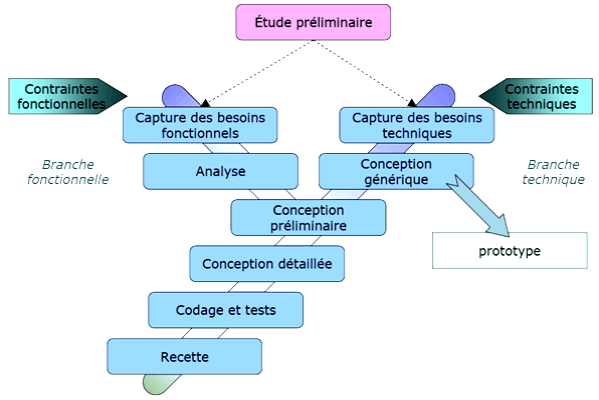
\includegraphics{./figure/illustrationDeveloppementEnY.png}
  \caption{Illustration du processus de développement en Y}
\end{figure}


% \begin{figure}[htbp]
%   \begin{tikzpicture}[node distance=2cm]
%     \tikzstyle{startstop} = [rectangle, rounded corners, minimum width=3cm, minimum height=1cm,text centered, draw=black, fill=gray!30]
%     \tikzstyle{process} = [rectangle, minimum width=3cm, minimum height=1cm, text centered, draw=black, fill=gray!10]
%     \tikzstyle{arrow} = [thick,->,>=stealth]
%     \tikzstyle{textblock} = [rectangle, text width=3cm, text centered]
%
%     % Nodes
%     \node (prelim) [startstop] {Étude préliminaire};
%     \node (functional) [textblock, left=2cm of prelim] {Contraintes fonctionnelles};
%     \node (technical) [textblock, right=2cm of prelim] {Contraintes techniques};
%     \node (funcReq) [process, below left=of prelim] {Capture des besoins fonctionnels};
%     \node (techReq) [process, below right=of prelim] {Capture des besoins techniques};
%     \node (analysis) [process, below=of funcReq] {Analyse};
%     \node (genericDesign) [process, below=of techReq] {Conception générique};
%     \node (prelimDesign) [process, below=of analysis, xshift=2cm] {Conception préliminaire};
%     \node (detailedDesign) [process, below=of prelimDesign] {Conception détaillée};
%     \node (coding) [process, below=of detailedDesign] {Codage et tests};
%     \node (testing) [process, below=of coding] {Recette};
%     \node (prototype) [process, right=of genericDesign, xshift=1cm] {Prototype};
%
%     % Arrows
%     \draw [arrow] (prelim) -- (funcReq);
%     \draw [arrow] (prelim) -- (techReq);
%     \draw [arrow] (funcReq) -- (analysis);
%     \draw [arrow] (techReq) -- (genericDesign);
%     \draw [arrow] (analysis) -- (prelimDesign);
%     \draw [arrow] (genericDesign) -- (prelimDesign);
%     \draw [arrow] (prelimDesign) -- (detailedDesign);
%     \draw [arrow] (detailedDesign) -- (coding);
%     \draw [arrow] (coding) -- (testing);
%     \draw [arrow] (genericDesign) -- (prototype);
%
%     % Text blocks
%     \node at (-3.5, -1) [textblock] {Branche fonctionnelle};
%     \node at ( 4.5, -1) [textblock] {Branche technique};
%
%   \end{tikzpicture}
%
% \end{figure}



\subsubsection{2TUP et UML}
L’utilisation de l’UML est étroitement liée au 2TUP. Les différents types de
diagrammes UML (diagramme de cas d’utilisation, de classes, de séquence et d’état)
sont largement utilisés tout au long du processus de développement pour modéliser
et documenter les besoins, les architectures, les interactions et les comportements
du système logiciel en cours de développement. L’UML fournit un langage visuel
standard et universellement accepté pour la représentation des systèmes logiciels.
Cela facilite la communication et la collaboration entre les membres de l’équipe
de développement et les
parties prenantes du projet.


\chapter{Analyse et conception}
Ce chapitre se concentre sur l’analyse approfondie des besoins de la plateforme
web et mobile pour la création collaborative et le partage d’arbres généalogiques
à \firm. Il présente également la conception de cette plateforme. L’analyse
approfondie des besoins est une étape importante dans le processus de développement,
car elle permet de définir clairement les fonctionnalités et les exigences
techniques nécessaires à la réalisation du projet. La conception, quant à elle,
vise à traduire ces besoins en solutions techniques efficaces et robustes.
Ce chapitre présentera donc en détail les besoins fonctionnels et techniques
identifiés lors de l’analyse, donnant ainsi les bases solides pour la conception de la plateforme.


\section{Analyse du besoin}
L'analyse du besoin vise à comprendre en profondeur les attentes et les exigences
des utilisateurs ainsi que les contraintes techniques et fonctionnelles qui
guideront le développement de la plateforme. Cette analyse repose sur une
étude approfondie des besoins fonctionnels et techniques.

\subsection{Besoins fonctionnels}
Les besoins fonctionnels définissent les fonctionnalités et les services que la
plateforme doit fournir à ses utilisateurs. Ils sont étroitement liés aux
objectifs et aux cas d’usage du système. Ces besoins incluent :

\begin{itemize}

  \item Création et gestion d’arbres généalogiques : les utilisateurs enregistrés
    peuvent créer, modifier et supprimer des arbres généalogiques et gérer les
    informations sur leurs proches;

  \item Consultation des arbres existants : les utilisateurs doivent pouvoir
    consulter les arbres généalogiques disponibles, y compris les détails sur
    les membres de leur famille;

  \item Recherche de membres de la famille : les utilisateurs doivent pouvoir
    trouver des personnes dans les arbres généalogiques existants sans avoir à
    créer de compte;

  \item Collaboration entre utilisateurs sur le même arbre : les utilisateurs
    enregistrés doivent pouvoir collaborer à la création et à la gestion d’un
    arbre généalogique, en y ajoutant, modifiant ou supprimant des informations
    sur les membres de la famille;

  \item Gestion des droits d’accès et de confidentialité : les utilisateurs doivent
    pouvoir déterminer qui aura accès aux arbres généalogiques qu’ils ont créés et
    gérés. Ils peuvent ainsi contrôler qui peut consulter, modifier ou contribuer
    aux informations contenues dans l’arbre;

  \item Partage et diffusion des arbres : les utilisateurs doivent pouvoir partager
    leurs arbres généalogiques avec leur famille et leurs proches.
    Ceux-ci auront alors accès à des versions consultables et visualisables.

\end{itemize}

\subsection{Besoins techniques}
Les besoins techniques décrivent les contraintes et les exigences liées à l’infrastructure
et aux technologies utilisées pour développer la plateforme. Cela inclut :

\begin{itemize}
  \item \textbf{Le choix des technologies de développement :} les langages de
    programmation, les frameworks et les outils qui seront utilisés pour créer
    la plateforme. Dans notre cas, nous utilisons :
    \begin{itemize}
      \item Langage de programmation : TypeScript (web et mobile)
      \item Frameworks : Next.js (web), Expo (mobile)
    \end{itemize}

  \item \textbf{La gestion des données :} la manière dont les informations sur les
    arbres généalogiques et les membres de la famille seront stockées, gérées
    et sécurisées. Les données sont stockées dans une base de données
    PostgreSQL. Prisma est utilisé pour gérer les opérations de base de
    données, assurant l'intégrité et la sécurité des données grâce à des
    schémas stricts et des migrations contrôlées. Et Docker est utilisé pour
    créer un conteneurs pour le \ac{SGBD};

  \item \textbf{L’interface utilisateur :} la conception de l’interface utilisateur
    pour garantir une expérience utilisateur intuitive et conviviale.
    Next.js est utilisé pour le rendu côté serveur et les pages réactives,
    assurant une performance élevée et une expérience utilisateur fluide;

  \item \textbf{La compatibilité et la sécurité :} la compatibilité avec les navigateurs
    web et les appareils mobiles, la sécurité des données, la scalabilité pour
    gérer un grand nombre d’utilisateurs, ainsi que l’interopérabilité avec
    d’autres systèmes et services existants. Les pages et composants sont
    testés pour être compatibles avec les principaux navigateurs
    (Chrome, Firefox, Safari) et optimisés pour les appareils mobiles. Docker
    permet de facilement scaler l'application pour gérer une augmentation du
    nombre d'utilisateurs. Les mesures de sécurité incluent l'utilisation de
    HTTPS, la gestion des sessions sécurisées, et des pratiques de développement
    sécurisées pour éviter les vulnérabilités courantes;

  \item \textbf{La gestion des erreurs :} la gestion des erreurs et des exceptions
    pour garantir la fiabilité et la robustesse de la plateforme. Les erreurs
    sont gérées de manière élégante et informative pour les utilisateurs, tout
    en étant enregistrées et surveillées pour permettre une résolution rapide
    des problèmes.

\end{itemize}

\section{Conception du système}
Dans cette section, nous aborderons les spécifications fonctionnelles du
système. Nous décrirons les acteurs impliqués, les cas d’utilisation identifiés,
ainsi que les relations et la classification de ces cas d’utilisation.

\subsection{Spécifications fonctionnelles}
Les spécifications fonctionnelles décrivent les fonctionnalités et les interactions
du système avec ses utilisateurs. Elles fournissent une vue détaillée des
besoins opérationnels du système.

\subsubsection{Identification des acteurs}
Les acteurs sont les entités externes qui interagissent avec le système.
Dans notre plateforme de création collaborative et de partage d'arbres
généalogiques à Mazala-Firm, les acteurs identifiés comprennent :

\begin{itemize}
  \item les membres;

  \item les administrateurs;

  \item et les visiteurs.

\end{itemize}

\subsubsection{Diagramme de contexte statique}
Le diagramme de contexte statique représente graphiquement les acteurs et leurs
relations avec le système. Il fournit une vue d’ensemble claire des interactions
entre les différentes entités impliquées dans notre plateforme de création
collaborative et de partage d’arbres généalogiques. Ce diagramme met en évidence
les liens essentiels entre les utilisateurs inscrits, les administrateurs du
système et les visiteurs non enregistrés, ce qui illustre la dynamique de
notre écosystème numérique.

\begin{figure}[htbp]
  \centering
  \begin{tikzpicture}[node distance=2cm, every node/.style={inner sep=3pt}]
    \node (system) [draw, rectangle, minimum width=2.5cm, text width=2cm, align=center] {Système};
    \node (utilisateurs) [above left=of system] {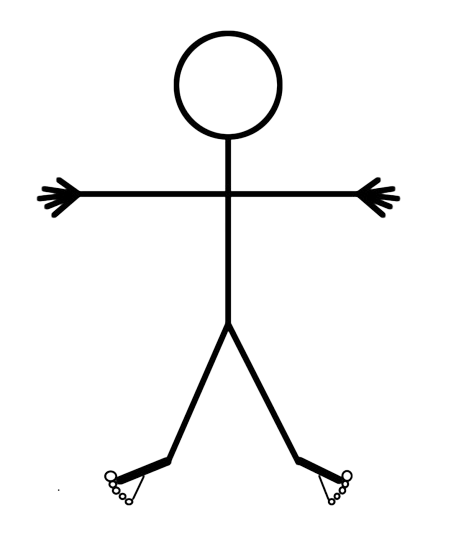
\includegraphics[width=1cm]{images/stickman.png}};
    \node (admins) [above right=of system] {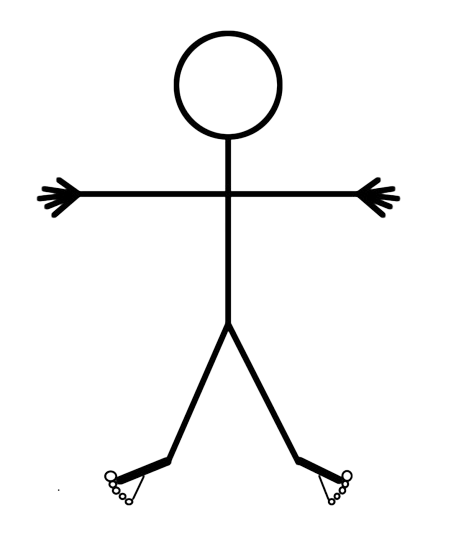
\includegraphics[width=1cm]{images/stickman.png}};
    \node (visiteurs) [below=of system] {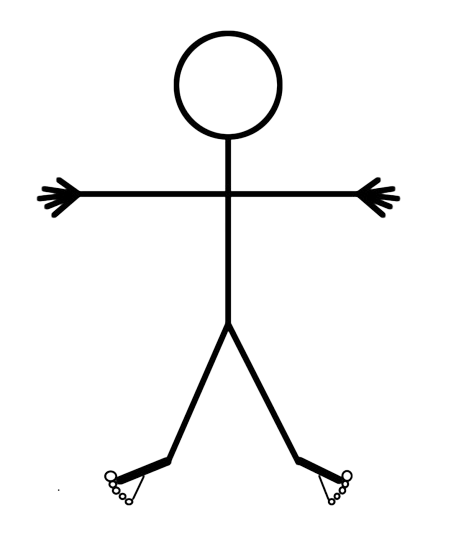
\includegraphics[width=1cm]{images/stickman.png}};

    \draw[->] (utilisateurs) -- node[anchor=south] {1..*} (system);
    \draw[->] (admins) -- node[anchor=east] {1..*} (system);
    \draw[->] (visiteurs) -- node[anchor=east] {1..*} (system);

    \node[right=0.3cm of utilisateurs] {Membre};
    \node[right=0.3cm of admins] {Administrateurs};
    \node[right=0.3cm of visiteurs] {Visiteurs};
  \end{tikzpicture}
  \caption{Diagramme de contexte statique}
\end{figure}


\subsubsection{Identification des cas d'utilisation}
Les cas d'utilisation décrivent les interactions entre les acteurs et le
système afin atteindre des objectifs spécifiques. Pour notre sytème, on retouve :

\begin{itemize}
  \item Gérer un arbre généalogique;

  \item Gérer des membres;

  \item Modifier les informations des membres;

  \item Consulter un arbre généalogique;

  \item Rechercher des membres de la famille;

  \item Accorder des droits d'accès et de confidentialité;

  \item Partager un arbre généalogique;

  \item Collaborer à la création d'un arbre généalogique;

  \item Gérer un profile;

  \item Administrer le système.

\end{itemize}


\subsubsection{Relation entre les cas d'utilisation (Use case)}
Pour affiner la représentation des interactions entre les différents cas
d’utilisation de notre système, nous utilisons les relations standardisées
définies par UML. Ces relations permettent de mieux comprendre les liens entre
les différentes fonctionnalités du système. Voici comment elles s’appliquent
dans notre contexte :

\begin{itemize}

  \item Inclusion (\say{include}) : cette relation est utilisée lorsqu’un cas
    d’utilisation de base incorpore explicitement un autre cas d’utilisation,
    de manière obligatoire. Dans notre système, nous pourrions par exemple
    inclure le cas d’utilisation \say {Modifier les informations des membres}
    dans le cas d’utilisation \say{Gérer des membres}, car la modification des
    informations des membres fait partie intégrante de la gestion des membres.

  \item Extension (\say{extend}) : cette relation est utilisée lorsqu’une
    utilisation de base incorpore implicitement un autre cas d’utilisation, de
    façon optionnelle. Par exemple, le cas d’utilisation \say{Partager un arbre généalogique}
    peut être étendu par le cas d’utilisation \say{Accorder des droits d’accès et de confidentialité}.
    Ainsi, lorsqu’un utilisateur souhaite partager un arbre généalogique, il a
    également la possibilité d’accorder des droits d’accès spécifiques à
    certains membres de sa famille.

  \item Généralisation/spécialisation : cette relation sert à décrire un lien
    du genre \say{est un} entre différents cas d’utilisation. Dans notre système,
    on peut trouver une généralisation entre les cas d’utilisation \say {Gérer un
    arbre généalogique} et \say{Gérer des membres}, puisque gérer un arbre
    généalogique inclut aussi la gestion des membres qui en font partie. Les
    fonctionnalités de gestion des membres peuvent donc être considérées comme
    une spécialisation du cas d’utilisation de gestion d’un arbre généalogique.

\end{itemize}


\newpage
\begin{figure}
  \begin{tikzpicture}

% Actors
\umlactor[x=-3, y=3]{Visiteur}
\umlactor[x=-3, y=1]{Membre}
\umlactor[x=-3, y=-2]{Admin}

% Use Cases
\begin{umlsystem}[x=0, y=0, fill=white]{Plateforme Mazala-Firm}
  \umlusecase[x=0, y=4]{Consulter arbre}
  \umlusecase[x=0, y=2]{Rechercher membres}
  \umlusecase[x=0, y=0]{Partager arbre}
  \umlusecase[x=5, y=4]{Gérer arbre}
  \umlusecase[x=5, y=2]{Gérer membres}
  \umlusecase[x=5, y=0]{Modifier infos}
  \umlusecase[x=10, y=4]{Collaborer arbre}
  \umlusecase[x=10, y=2]{Accorder droits}
  \umlusecase[x=10, y=0]{Gérer profil}
  \umlusecase[x=10, y=-2]{Administrer}
\end{umlsystem}

% Associations
\umlassoc{Visiteur}{usecase-1}
\umlassoc{Visiteur}{usecase-2}
\umlassoc{Membre}{usecase-3}
\umlassoc{Membre}{usecase-4}
\umlassoc{Membre}{usecase-5}
\umlassoc{Membre}{usecase-6}
\umlassoc{Membre}{usecase-7}
\umlassoc{Membre}{usecase-8}
\umlassoc{Membre}{usecase-9}
\umlassoc{Admin}{usecase-10}

% Relationships
\umlinclude{usecase-4}{usecase-5}
\umlinclude{usecase-5}{usecase-6}
\umlVHextend{usecase-3}{usecase-8}
\umlinherit{usecase-5}{usecase-4}

\end{tikzpicture}
  \caption{Diagramme de cas d'utilisation}
\end{figure}

\subsubsection{Classification des cas d'utilisation (priorités, risques et itérations)}
Dans cette section, nous classons les cas d’utilisation identifiés selon leur
priorité, leur niveau de risque et leur inclusion dans les itérations du
développement. Cette classification servira à guider la planification et
l’exécution du projet en mettant en évidence les fonctionnalités les plus
importantes, les risques potentiels à surveiller et les étapes itératives du
développement.

\begin{table}[htbp]
  \centering
  \begin{tabularx}{\textwidth}{|l|l|l|X|}
    \hline
    \textbf{Cas d'utilisation} & \textbf{Priorité} & \textbf{Risque} & \textbf{Itération} \\ \hline
    Gérer un arbre généalogique & Forte & Moyen & 1 \\ \hline
    Gérer des membres & Forte & Moyen & 1 \\ \hline
    Modifier les informations des membres & Moyenne & Faible & 1 \\ \hline
    Consulter un arbre généalogique & Forte & Faible & 1 \\ \hline
    Rechercher des membres de la famille & Moyenne & Moyen & 2 \\ \hline
    Accorder des droits d’accès et de confidentialité & Moyenne & Élevé & 2 \\ \hline
    Partager un arbre généalogique & Forte & Élevé & 2 \\ \hline
    Collaborer à la création d’un arbre généalogique & Forte & Élevé & 3 \\ \hline
    Gérer un profil & Moyenne & Moyen & 3 \\ \hline
    Administrer le système & Moyenne & Élevé & 3 \\ \hline
  \end{tabularx}
  \caption{Classification des cas d'utilisation en fonction de la priorité, du risque et de l'itération}
\end{table}

Dans le tableau ci-dessus, chaque cas d’utilisation est évalué selon trois critères principaux :

\begin{itemize}

  \item Priorité : indique l’importance relative du cas d’utilisation pour
    l’achèvement du projet. Les priorités peuvent être classées comme forte, moyennes ou basses.

  \item Risque : évalue le niveau de risque associé à la mise en œuvre du cas
    d’utilisation. Les risques peuvent être classés comme faibles, moyens ou élevés.

  \item Itération : indique dans quelle itération du développement le cas
    d’utilisation sera implémenté. Les itérations peuvent être numérotées séquentiellement.

\end{itemize}

Cette classification constituera un outil précieux pour la planification et la
gestion du projet. Elle permettra une allocation efficace des ressources et
une identification proactive des risques potentiels.

\newpage

\subsection{Spécification détaillée }
Dans cette section, nous fournissons une spécification détaillée des cas
d’utilisation identifiés. Nous décrivons les interactions entre les acteurs et
le système, ainsi que les flux d’événements associés.

\subsubsection{Description textuelle d'un cas d'utilisation}
\textbf{Cas d’utilisation :} Gérer un arbre généalogique

\textbf{Acteur :} Utilisateur enregistré

\textbf{Autres acteurs :} Système

\textbf{Description :} Ce cas d’utilisation permet à l’utilisateur de créer,
de modifier, de visualiser et de supprimer des arbres généalogiques.

\textbf{Préconditions :} L’utilisateur est authentifié et peut accéder à la
fonctionnalité de gestion des arbres généalogiques.

\textbf{Postconditions :} Les modifications apportées à l'arbre généalogique
sont enregistrées dans le système.

\textbf{Séquencement des événements}

Le cas d’utilisation commence lorsque l’utilisateur se connecte à la plateforme
et desire gérer un arbre généalogique.

\textbf{Scénario nominal :}

\begin{enumerate}

  \item  L’utilisateur se connecte à l’application.

  \item Le système affiche alors une barre de navigation latérale comportant un
    bouton \say{Créer un arbre} ainsi qu’une liste d’arbres généalogiques déjà
    existants chez cet utilisateur.

  \item L’utilisateur peut ensuite sélectionner parmi les options suivantes :
    \begin{itemize}
      \item Créer un nouvel arbre généalogique;
      \item Modifier un arbre généalogique existant;
      \item Consulter un arbre généalogique existant;
      \item Supprimer un arbre généalogique existant;
      \item Visualiser un arbre généalogique existant.
    \end{itemize}

  \item Si l’utilisateur décide de créer un nouvel arbre généalogique :
    \begin{enumerate}
      \item il doit cliquer sur le bouton \say{Créer un nouvel arbre};
      \item le système affiche une fenêtre où il devra entrer un nom et un type(publique, privé)
        pour son nouvel arbre généalogique;
      \item l’utilisateur valide ses informations;
      \item le système crée alors un nouvel arbre généalogique et l’affiche dans la liste des arbres
        généalogiques de l’utilisateur.
    \end{enumerate}

  \item  Si l’utilisateur décide de modifier un arbre généalogique existant :
    \begin{enumerate}
      \item il sélectionne l’arbre généalogique dans la barre de navigation latérale.;
      \item le système affiche alors les détails de l’arbre généalogique sélectionné;
      \item utilisateur effectue les modifications nécessaires (ajouts,
        suppressions, modifications de membres ou de relations) ou les
        informations de l’arbre généalogique;

        \subitem Pour ajouter un membre :

          \begin{itemize}
            \item l’utilisateur clique sur l’option \say{Ajouter un membre};
            \item le e système présente un formulaire qui demande des
              renseignements au sujet du nouveau membre (son nom, sa date de
              naissance, ses relations, etc.);
            \item l’utilisateur remplit les champs requis et valide son entrée;
            \item le système ajoute le nouveau membre à l’arbre généalogique;
          \end{itemize}

        \subitem Pour modifier les informations de l’arbre généalogique :

          \begin{itemize}
            \item l’utilisateur clique sur l’option \say{Modifier les informations};
            \item le système affiche un formulaire de modification des informations de l’arbre généalogique;
            \item l’utilisateur effectue les modifications nécessaires et valide ses changements;
            \item le système enregistre les modifications apportées à l’arbre généalogique.
          \end{itemize}

      \item le système sauvegarde toutes les modifications apportées à l’arbre généalogique.
    \end{enumerate}

  \item Si l’utilisateur souhaite consulter, un arbre généalogique existant :
    \begin{enumerate}
      \item il sélectionne l’arbre généalogique dans la barre de navigation latérale;
      \item le système affiche alors l’arbre généalogique sélectionné avec les
        informations sur ses membres et leurs liens.
    \end{enumerate}

  \item Si l’utilisateur souhaite supprimer un arbre généalogique existant :
    \begin{enumerate}
      \item il sélectionne l’arbre généalogique dans la barre de navigation latérale;
      \item le système demande une confirmation avant de procéder à la
        suppression définitive de l’arbre généalogique;
      \item si l’utilisateur accepte, le système efface l’arbre généalogique
        ainsi que toutes les données connexes de la liste dans la barre de
        navigation latérale.
    \end{enumerate}

\end{enumerate}

\textbf{Scénario alternatif :}

\subsubsection*{Scénarios alternatifs}

\begin{enumerate}
    \item \textbf{Scénario alternatif pour la création d'un arbre généalogique :}
    \begin{itemize}
        \item \textbf{Étape 4a :} L'utilisateur tente de créer un arbre
          généalogique mais ne saisit pas un nom valide ou ne choisit pas un type.
        \begin{itemize}
            \item le système affiche un message d'erreur demandant de saisir
              un nom valide ou de choisir un type;
            \item l'utilisateur saisit un nom valide ou choisit un type et confirme;
            \item Le système crée le nouvel arbre généalogique et l'ajoute à la liste.
        \end{itemize}
    \end{itemize}

    \item \textbf{Scénario alternatif pour la modification d'un arbre généalogique :}
    \begin{itemize}
        \item \textbf{Étape 5a :} L'utilisateur tente d'ajouter un membre mais
          laisse des champs obligatoires vides.
        \begin{itemize}
            \item le système affiche un message d'erreur demandant de compléter les champs obligatoires;
            \item l'utilisateur complète les informations manquantes et confirme;
            \item le système ajoute le nouveau membre à l'arbre généalogique.
        \end{itemize}
    \end{itemize}

    \item \textbf{Scénario alternatif pour la suppression d'un arbre généalogique :}
    \begin{itemize}
        \item \textbf{Étape 7a :} L'utilisateur sélectionne un arbre généalogique à supprimer mais change d'avis et annule l'opération.
        \begin{itemize}
            \item Le système annule l'opération de suppression et revient à la liste des arbres généalogiques.
        \end{itemize}
    \end{itemize}

    \item \textbf{Scénario alternatif pour la visualisation d'un arbre généalogique :}
    \begin{itemize}
        \item \textbf{Étape 6a :} L'utilisateur tente de visualiser un arbre
          généalogique mais celui-ci contient des erreurs de données (ex. : relations incorrectes).
        \begin{itemize}
            \item le système affiche un message d'erreur et propose des options de correction.
            \item l'utilisateur corrige les erreurs et le système affiche l'arbre généalogique mis à jour.
        \end{itemize}
    \end{itemize}

\end{enumerate}

\textbf{Scénario d'exception :}
\begin{enumerate}
  \item Si, à l’étape 3, l’utilisateur ferme la barre de navigation latérale
    ,le scénario principal est interrompu.

  \item Si l’utilisateur essaie de supprimer un arbre généalogique sans avoir
    obtenu de confirmation, le système annule
\end{enumerate}

Cette description textuelle fournit une vue détaillée des étapes et des
interactions impliquées dans le cas d’utilisation \say{Gérer un arbre généalogique}.
Cela permet une compréhension claire des fonctionnalités offertes par ce cas
d’utilisation.


\subsubsection{Diagramme de séquence}

Le diagramme de séquence est un outil visuel permettant de représenter les
interactions entre les acteurs et le système dans un scénario donné. Il montre
la séquence des messages échangés entre les objets du système au cours d’un
scénario d’exécution. Dans notre cas, nous allons illustrer le scénario de
création et de suppression d’un arbre généalogique par un utilisateur.



\begin{center}
  \newpage
  \textbf{Gestion d'un arbre généalogique}

  \begin{figure}[htbp]
    \centering
    \begin{sequencediagram}

      \newthread{user}{Utilisateur}
      \newinst[7]{sys}{Système}  % Adjusting the distance here

      \begin{sdblock}{Connexion}{}
        \begin{call}{user}{Se connecter}{sys}{Page de connexion}
          \mess{sys}{Afficher page de connexion}{user}
          \begin{call}{user}{Entrer identifiants}{sys}{Authentifier}
            \mess{sys}{Valider identifiants}{user}
          \end{call}
        \end{call}
      \end{sdblock}

      \begin{sdblock}{Opérations sur Arbre Généalogique}{}
        \begin{call}{user}{Sélectionner une action CRUD}{sys}{Afficher page correspondante}
          \begin{call}{user}{Entrer ou confirmer les détails}{sys}{Valider l'opération}
            \mess{sys}{Mettre à jour la base de données et afficher le résultat}{user}
          \end{call}
        \end{call}
      \end{sdblock}

    \end{sequencediagram}

    \caption{Diagramme de séquence pour gestion d'un arbre généalogique}
  \end{figure}

\end{center}

\subsubsection{Diagramme d'activité}

Le diagramme d’activité est un outil visuel qui permet de représenter le flux
de contrôle entre les différentes activités d’un système. Il montre comment les
activités sont organisées et enchaînées pour atteindre un objectif spécifique.
Dans notre cas, nous allons illustrer le processus d’ajout d’un membre à un
arbre de la famille dans un arbre généalogique.
% \tikzstyle{startstop} = [rectangle, rounded corners, minimum width=3cm, minimum height=1cm, text centered, draw=black, fill=red!30]
% \tikzstyle{process} = [rectangle, minimum width=3cm, minimum height=1cm, text centered, draw=black, fill=orange!30]
% \tikzstyle{decision} = [diamond, minimum width=3cm, minimum height=1cm, text centered, draw=black, fill=green!30]
% \tikzstyle{arrow} = [thick,->,>=stealth]

% \tikzstyle{startstop} = [draw, circle, rounded corners, minimum width=1cm, minimum height=1cm, text centered, draw=black]
% \tikzstyle{process} = [rectangle, minimum width=3cm, minimum height=1cm, text centered, draw=black]
% \tikzstyle{decision} = [diamond, minimum width=3cm, minimum height=1cm, text centered, draw=black]
% \tikzstyle{arrow} = [thick,->,>=stealth]


\begin{figure}[htbp]
  \centering
  \tikzstyle{startstop} = [draw, circle, fill=black, text=white, minimum width=1cm, minimum height=1cm, text centered, draw=black]
  \tikzstyle{stop} = [draw, circle, minimum width=1cm, minimum height=1cm, text centered, draw=black, path picture={
    \draw[black, thick] (path picture bounding box.south west) -- (path picture bounding box.north east);
    \draw[black, thick] (path picture bounding box.north west) -- (path picture bounding box.south east);
  }]
  \tikzstyle{process} = [rectangle, minimum width=3cm, minimum height=1cm, text centered, draw=black]
  \tikzstyle{decision} = [diamond, minimum width=1cm, minimum height=1cm, text centered, draw=black]
  \tikzstyle{arrow} = [thick,->,>=stealth]
  \begin{tikzpicture}[node distance=2cm]

    \node (start) [startstop] {Début};
    \node (login) [process, below of=start] {Se connecter};
    \node (displayNav) [process, below of=login] {Afficher barre de navigation};
    \node (selectTree) [decision, below of=displayNav] {};
    \node (firstStop) [startstop, right=3cm of selectTree] {Fin};
    \node (fillForm) [process, below of=selectTree, yshift=-1cm] {Entrer ou confirmer les détails};
    \node (validate) [decision, below of=fillForm, yshift=-1cm] {};
    \node (saveMember) [process, below of=validate, yshift=-1cm] {Sauvegarder le membre};
    \node (stop) [startstop, below of=saveMember] {Fin};

    \draw [arrow] (start) -- (login);
    \draw [arrow] (login) -- (displayNav);
    \draw [arrow] (displayNav) -- (selectTree);
    \draw [arrow] (selectTree) -- node[anchor=east] {Oui} (fillForm);
    \draw [arrow] (selectTree) -- node[anchor=south] {Non} (firstStop);
    \draw [arrow] (fillForm) -- (validate);
    \draw [arrow] (validate) -- node[anchor=east] {Oui} (saveMember);
    \draw [arrow] (saveMember) -- (stop);
    \draw [arrow] (validate.east) -- ++(3,0) |- node[anchor=center] {Non} (firstStop);

    \node[left=0.3cm of selectTree] {Choix d'une action};
    \node[left=0.3cm of selectTree] {Choix d'une action};
    \node[left=0.3cm of validate] {Validate ?};

  \end{tikzpicture}
  \caption{Diagramme d'activité pour la gestion d'un arbre généalogique}
\end{figure}


\newpage
\subsection{Réalisations des cas d'utilisation}
Dans cette section, nous abordons la mise en œuvre concrète des cas
d’utilisation identifiés précédemment. À ce stade, nous traduisons les
interactions entre les acteurs et le système en fonctionnalités opérationnelles.
Nous détaillons également les règles de gestion spécifiques qui guident le
comportement du système lors de l’exécution de chaque cas d’utilisation. Enfin,
nous présentons le modèle du domaine sous forme d’un diagramme de classe du
système, offrant ainsi une vue structurée des entités et de leurs relations
au sein du système.
\subsubsection{Quelques règles de gestion}

Nous allons établir ici un ensemble de règles de gestion qui régissent le
comportement des fonctionnalités mises en œuvre. Ces règles définissent les
contraintes et les conditions d’exécution pour garantir la cohérence et la
fiabilité des opérations réalisées par le système.

\begin{itemize}
  \item \textbf{Règle de gestion 1 :} Un utilisateur ne peut pas modifier un arbre généalogique qui ne lui appartient pas.
  \item \textbf{Règle de gestion 2 :} Un arbre généalogique ne peut pas être partagé avec des utilisateurs non enregistrés.
  \item \textbf{Règle de gestion 3 :} Un arbre généalogique privé ne peut être consulté que par son propriétaire.
  \item \textbf{Règle de gestion 4 :} Un arbre généalogique publique peut être consulté par tous les utilisateurs enregistrés.
  \item \textbf{Règle de gestion 5 :} Un arbre généalogique ne peut pas être supprimé s’il contient des membres.
  \item \textbf{Règle de gestion 6 :} Un arbre généalogique ne peut pas être partagé avec des utilisateurs qui n’ont pas de compte.
\end{itemize}

\subsubsection{Modele du domaine (Diagramme de classe du système)}
Le diagramme de classe du système est une représentation visuelle des
entités principales du domaine et de leurs relations. Il offre une vue
d'ensemble de la structure du système, en mettant en évidence les différentes
classes d'objets, leurs attributs et leurs associations. Cette représentation
facilite la compréhension des concepts clés du domaine et guide la conception
de la solution logicielle.


\newpage
\begin{figure}[htbp]
  \begin{tikzpicture}

    % User class
    \umlclass{Utilisateur}{
      + id : String \\
      + nomUtilisateur : String \\
      + email : String \\
      + MdpHaché : String \\
      + DateCreation : DateTime \\
      + DateModifier : DateTime
    }{
      + créerArbre() : void \\
      + modifierArbre() : void \\
      + supprimerArbre() : void \\
      + visualiserArbre() : void
    }

    % Profile class
    \umlclass[x=0, y=-6]{Profil}{
      + id : String \\
      + prénom : String \\
      + nom : String \\
      + avatarURL : String
    }{}

    % UserAccess class
    \umlclass[x=7, y=-5]{AccèsUtilisateur}{
      + id : String \\
      + level : NiveauAccès \\
      + userExternalId : String \\
      + treeId : String
    }{}

    % Tree class
    \umlclass[x=7, y=-10]{Arbre}{
      + id : String \\
      + name : String \\
      + type : TypeArbre
    }{
      + ajouterMembre() : void \\
      + modifierMembre() : void \\
      + supprimerMembre() : void
    }

    % Member class
    \umlclass[x=0, y=-10]{Membre}{
      + id : String \\
      + firstname : String \\
      + nom : String \\
      + dateNaissance : DateTime \\
      + lieuNaissance : String \\
      + sexe : Sexe \\
      + avatarURL : String \\
      + description : String
    }{}

    % Relation class
    \umlclass[x=0, y=-16]{Relation}{
      + idPapa : String \\
      + idMaman : String \\
      + conjoints : String[] \\
      + enfants : String[] \\
      + idMembre : String
    }{}

    % Enums
    \umlenum[x=14, y=-5]{NiveauAccès}{
      admin \\
      editeur \\
      lecteur
    }

    \umlenum[x=14, y=-10]{TypeArbre}{
      publique \\
      privé
    }

    \umlenum[x=14, y=-15]{Sexe}{
      masculin \\
      feminin
    }

    % Aggregations and Compositions
    \umluniaggreg[mult1=1, pos1=0.7, mult2=0..1, pos2=0.3]{Utilisateur}{Profil}
    \umluniaggreg[mult1=1, pos1=0.7, mult2=*, pos2=0.3]{Utilisateur}{AccèsUtilisateur}
    \umluniaggreg[mult1=1, pos1=0.7, mult2=*, pos2=0.3]{Arbre}{Membre}
    \umluniaggreg[mult1=1, pos1=0.7, mult2=*, pos2=0.3]{Arbre}{AccèsUtilisateur}
    \umlunicompo[mult1=1, pos1=0.7, mult2=0..1, pos2=0.3]{Membre}{Relation}

    % Relationships
    \umluniassoc[mult1=1, pos1=0.7, mult2=1, pos2=0.3]{Profil}{Utilisateur}
    \umluniassoc[mult1=1, pos1=0.7, mult2=*, pos2=0.3]{AccèsUtilisateur}{Utilisateur}
    \umluniassoc[mult1=1, pos1=0.7, mult2=*, pos2=0.3]{AccèsUtilisateur}{Arbre}
    \umluniassoc[mult1=1, pos1=0.7, mult2=*, pos2=0.3]{Membre}{Arbre}
    \umluniassoc[mult1=1, pos1=0.7, mult2=1, pos2=0.3]{Relation}{Membre}

    % Enum Relations
    \umluniassoc[mult1=1, pos1=0.7, mult2=*, pos2=0.3]{AccèsUtilisateur}{NiveauAccès}
    \umluniassoc[mult1=1, pos1=0.7, mult2=*, pos2=0.3]{Arbre}{TypeArbre}
    \umluniassoc[mult1=1, pos1=0.7, mult2=*, pos2=0.3]{Membre}{Sexe}

  \end{tikzpicture}
  \caption{Diagramme de classe du système}
\end{figure}


\subsubsection{Diagramme d'objet}
Un diagramme d’objet représente graphiquement les objets et leurs relations à
un moment donné. À l’inverse du diagramme de classe, qui décrit la structure
statique des classes et de leurs relations dans un système, le diagramme
d’objet illustre des instances spécifiques des classes (objets) et les liens
entre eux dans un contexte particulier. Il est utilisé pour visualiser l’état
d’un système à un instant précis, facilitant la compréhension des interactions
dynamiques et des configurations temporaires des objets.

\begin{figure}[htbp]
    \centering
    \begin{tikzpicture}[
        object/.style={rectangle, draw, text width=6cm, minimum height=1cm, align=left, font=\ttfamily},
        attribute/.style={text width=7cm, align=left, font=\ttfamily}
    ]

        % Object instances
        \node[object] (utilisateur1) {
            \textbf{Utilisateur: utilisateur1} \\
            \underline{id} = "u1234" \\
            \underline{nomUtilisateur} = "jdoe" \\
            \underline{email} = "jdoe@example.com" \\
            \underline{MdpHaché} = "******" \\
            \underline{DateCreation} = "2022-01-01" \\
            \underline{DateModifier} = "2022-02-01"
        };

        \node[object, below=of utilisateur1] (profile1) {
            \textbf{Profil: profile1} \\
            \underline{id} = "p1234" \\
            \underline{prénom} = "John" \\
            \underline{nom} = "Doe" \\
            \underline{avatarURL} = "http://example.com/avatar.jpg"
        };

        \node[object, right=of utilisateur1] (acces1) {
            \textbf{AccèsUtilisateur: acces1} \\
            \underline{id} = "a1234" \\
            \underline{level} = "admin" \\
            \underline{userExternalId} = "u1234" \\
            \underline{treeId} = "t1234"
        };

        \node[object, below=of acces1] (arbre1) {
            \textbf{Arbre: arbre1} \\
            \underline{id} = "t1234" \\
            \underline{name} = "Doe Family Tree" \\
            \underline{type} = "privé"
        };

        \node[object, below=of profile1] (member1) {
            \textbf{Membre: member1} \\
            \underline{id} = "m1234" \\
            \underline{firstname} = "Jane" \\
            \underline{nom} = "Doe" \\
            \underline{dateNaissance} = "1990-01-01" \\
            \underline{lieuNaissance} = "Paris" \\
            \underline{sexe} = "féminin" \\
            \underline{avatarURL} = "http://example.com/jane.jpg" \\
            \underline{description} = "Daughter of John Doe"
        };

        \node[object, below=of member1] (relation1) {
            \textbf{Relation: relation1} \\
            \underline{idPapa} = "m1234" \\
            \underline{idMaman} = "m1235" \\
            \underline{conjoints} = ["m1236"] \\
            \underline{enfants} = ["m1237"] \\
            \underline{idMembre} = "m1234"
        };

        % Relationships
        \draw[->] (utilisateur1) -- (profile1);
        \draw[->] (utilisateur1) -- (acces1);
        \draw[->] (acces1) -- (arbre1);
        \draw[->] (arbre1) -- (member1);
        \draw[->] (member1) -- (relation1);

    \end{tikzpicture}
    \caption{Diagramme d'objet du système}
\end{figure}


\newpage
\subsection{Conception architecturale}
La conception architecturale est une étape importante du développement logiciel
qui vise à définir la structure globale d’un système et de ses composants
principaux. Elle comprend l’organisation des modules, la communication entre
eux et les contraintes techniques à respecter. Cette phase permet de créer une
base solide pour le développement, afin d’assurer que les exigences
fonctionnelles et non fonctionnelles seront satisfaites. La conception
architecturale se décline en plusieurs sous-sections, notamment l’architecture
logicielle et l’architecture globale de la solution.

\subsubsection{Architecture logicielle}
L’architecture logicielle décrit la structure organisationnelle d’un système
logiciel, y compris ses modules, leurs responsabilités et les interactions
entre eux. Elle vise à garantir la cohérence, la performance, la maintenabilité
et la scalabilité du système. L’architecture logicielle est un guide pour les
développeurs qui permet d’aligner les décisions techniques avec les objectifs
métier et les contraintes du projet.

Pour notre projet, nous avons opté pour une architecture basée sur plusieurs
patterns et concepts pour structurer nos applications.

\begin{itemize}
  \item \textbf{Architecture pour l'application web }

    Notre architecture se distingue par sa capacité à offrir un rendu côté
    serveur (SSR - Server-Side Rendering) ainsi que des pages statiques générées
    à la compilation (SSG - Static Site Generation). Cela améliore à la fois
    les performances et l’optimisation pour les moteurs de recherche (SEO).

    En outre, cette architecture permet de séparer les pages, les composants et
    les API, offrant ainsi une organisation plus claire et modulable.

  \item \textbf{Architecture pour l'application mobile}

    Notre architecture offre une expérience de développement simplifiée. Elle
    permet de développer des applications mobiles rapidement et efficacement grâce
    à des outils intégrés pour la gestion de la configuration, l’accès aux API
    natives, et les mises à jour en direct (OTA — Over-The-Air).

    Enfin, elle permet de séparer les vues, les composants et les services, offrant
    ainsi une organisation claire et modulaire des éléments de l’application.

    Cette approche optimise le développement cross-plateforme en utilisant une seule
    base de code pour les applications iOS et Android, tout en garantissant une
    expérience utilisateur native de haute qualité.
\end{itemize}



\subsubsection{Architecture globale de la solution (Diagramme de déploiement)}
L’architecture globale de la solution est souvent illustrée par un diagramme de
déploiement qui montre la configuration physique des composants logiciels sur
le matériel. Ce diagramme détaille comment les éléments logiciels sont
distribués à travers différents nœuds de réseau, tels que serveurs, bases de
données, et terminaux utilisateurs. Il aide à comprendre les aspects de
performance, de sécurité et de scalabilité de la solution, en montrant comment
les composants interagissent dans un environnement réel.

Dans notre cas, la plateforme pour la création collaborative et le partage
d’arbres généalogiques sont basés sur une architecture distribuée qui
comprend plusieurs composants clés.

Une architecture distribuée  désigne un système d'information ou un réseau pour
lequel l'ensemble des ressources disponibles ne se trouvent pas au même endroit
ou sur la même machine (\textcite{frwiki:212787328}).

% \begin{figure}[htbp]
%   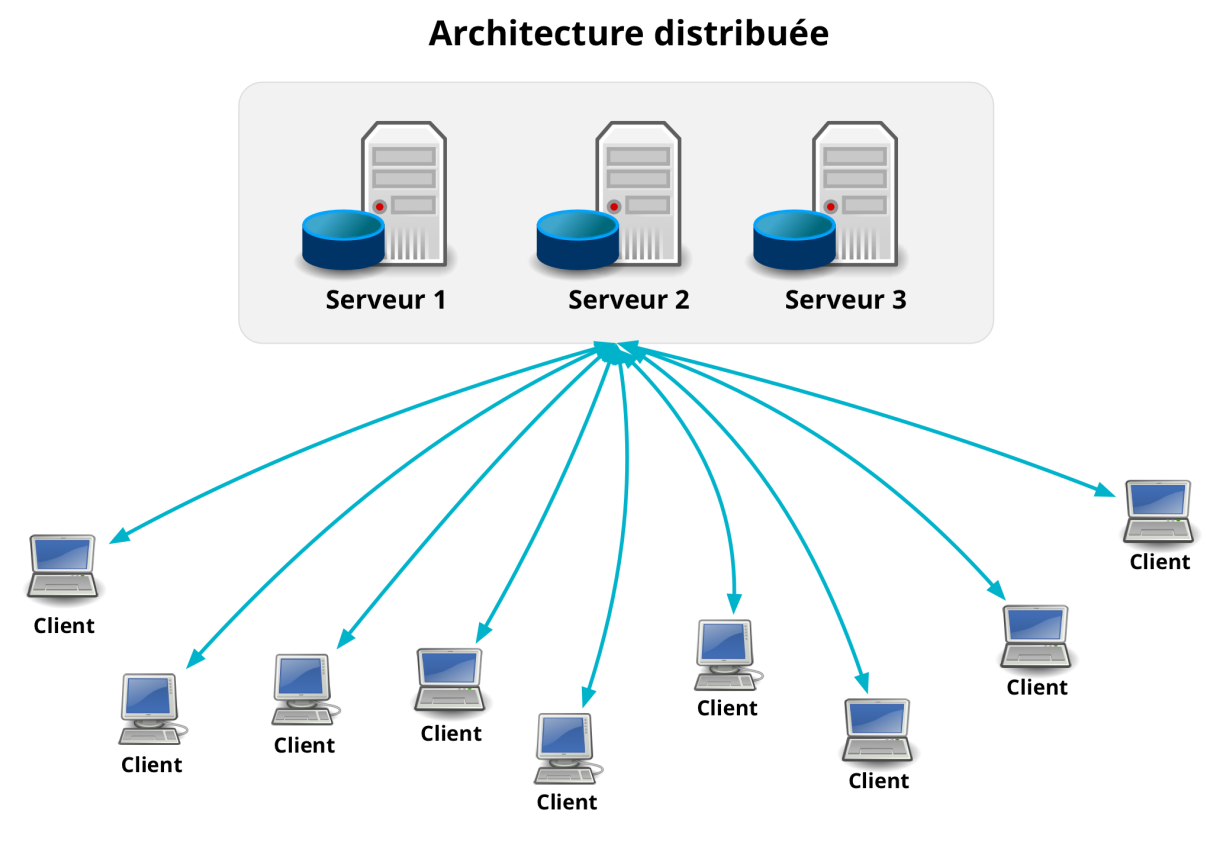
\includegraphics{images/architectureDistribuee.png}
%   \caption{Illustration de l'architecture distribuée }
% \end{figure}

\begin{itemize}
  \item \textbf{ Serveur Web :} Héberge l'application Next.js pour le rendu
    côté serveur (SSR) et le serveur API. Utilise Node.js pour exécuter le
    code JavaScript côté serveur.

  \item \textbf{Serveur de bases de données :} utilise PostgreSQL comme SGBD
    pour stocker les données relatives aux utilisateurs, aux arbres
    généalogiques et aux collaborations.

  \item \textbf{ Terminal utilisateur :} comprend les navigateurs Web pour
    accéder à l’application web Next.js et les applications mobiles Expo/React
    Native pour l’accès mobile.

  \item \textbf{Services externes :} intègre éventuellement des services
    externes pour des fonctionnalités supplémentaires, telles que
    l’authentification OAuth, le stockage de fichiers et les
    services de messagerie.

\end{itemize}

Voici un diagramme de déploiement illustrant cette architecture :

\begin{figure}[htbp]
  \centering
    \begin{tikzpicture}[
        server/.style={rectangle, draw, fill=blue!20, text centered, minimum height=2em, minimum width=4em},
        database/.style={cylinder, draw, shape border rotate=90, aspect=0.25, text centered, minimum height=2em, minimum width=4em},
        user/.style={ellipse, draw, fill=yellow!20, text centered, minimum height=2em, minimum width=4em},
        external/.style={rectangle, draw, dashed, fill=green!20, text centered, minimum height=2em, minimum width=4em},
        arrow/.style={->, thick, shorten <=2pt, shorten >=2pt}
    ]

    % Nodes
    \node[server] (webserver) {Serveur Web(Next.js/Node.js)};
    \node[database, below=of webserver, yshift=-2cm] (database) {Base de Données(PostgreSQL)};
    \node[user, left=of webserver, xshift=-1cm] (browser) {Navigateur};
    \node[user, right=of webserver, xshift=1cm] (mobileapp) {Application Mobile};
    \node[external, below=of database, yshift=-1cm] (auth) {Service d'authentification(OAuth)};

    % Arrows
    \draw[arrow] (browser) -- (webserver);
    \draw[arrow] (webserver) -- ( browser);
    \draw[arrow] (mobileapp) -- (webserver);
    \draw[arrow] (webserver) -- (mobileapp);
    \draw[arrow] (webserver) -- (database);
    \draw[arrow] (webserver) -- (auth);
    \draw[arrow] (auth) -- (webserver);

    \end{tikzpicture}
    \caption{Diagramme de déploiement}
\end{figure}

\newpage
\textbf{Avantages de cette architecture }

\begin{itemize}
  \item \textbf{Scalabilité:} les composants peuvent être mis à l’échelle
    indépendamment en fonction de la demande.

  \item \textbf{Sécurité :} la séparation des préoccupations permet
    d’améliorer la sécurité, notamment en isolant la base de données
    du reste de l’application.

  \item \textbf{Performance :} l'utilisation du rendu côté serveur et de la
    génération de pages statiques améliore la vitesse de chargement des
    pages et l’expérience utilisateur.

  \item \textbf{Maintenabilité :} l’architecture distribuée permet d’intégrer
    de nouveaux services et de mettre à jour les composants sans affecter
    l’ensemble du système.

\end{itemize}


\part{Evaluation et Réalisation}
\label{part:evaluation-et-realisation}
\chapter{Evaluation du projet}
Ce chapitre traite de l’organisation et de la gestion du projet, en analysant
les éléments clés nécessaires à une évaluation efficace.

\section{Organisation du projet}
L’organisation du projet implique la définition des rôles, des responsabilités
et des processus de travail. Une structure organisationnelle claire facilite
la coordination et la communication entre les membres de l’équipe, assurant
ainsi une progression harmonieuse du projet.

% Dans le cadre de ce projet, l’organisation est structurée autour de deux
% principaux processus : le processus de développement et le processus de
% validation.
%
% \begin{table}[htbp]
%   \centering
%   \begin{tabularx}{\textwidth}{|l|X|}
%     \hline
%     \textbf{Processus} & \textbf{Phases} \\ \hline
%     \multirow{4}{*}{Développement} & Analyse des besoins : Définir les fonctionnalités nécessaires à la création collaborative et au partage d’arbres généalogiques. \\
%      & Conception : Concevoir l'architecture logicielle de la solution, ainsi que l'interface utilisateur pour le web et le mobile. \\
%      & Développement : Implémenter les fonctionnalités selon les spécifications définies lors de l'analyse et de la conception. \\
%      & Tests : Réaliser des tests unitaires et d'intégration pour garantir le bon fonctionnement de l'application. \\ \hline
%     \multirow{2}{*}{Validation} & Vérification : Vérifier que les fonctionnalités implémentées répondent aux besoins et aux spécifications du projet. \\
%      & Validation : Valider l'application avec les utilisateurs finaux pour recueillir leurs retours et effectuer les ajustements nécessaires. \\ \hline
%   \end{tabularx}
%   \caption{Organisation du projet}
% \end{table}

\section{Intervenant}

\begin{table}[htbp]
  \centering
  \begin{tabularx}{\textwidth}{|l|l|X|}
    \hline
    \textbf{Intervenants} & \textbf{Fonctions} & \textbf{Rôles} \\ \hline
    M. Christopher BANDZOUZI & Ingénieur Informaticien & Directeur de projet  \\ \hline
    M. Samuel Exaucé NANDI & Etudiant & Réalisateur \\ \hline
    M. Dieu-Veille Frédy ONIANGUE-DESO & Etudiant & Réalisateur \\ \hline
    Me. Rovélia MOUNTOU & Sécrétaire Mazala-Firm & Tutrice de stage \\ \hline
  \end{tabularx}
  \caption{Intervenants}
\end{table}

\section{Planification des tâches}
La planification des tâches consiste à décomposer le projet en activités
distinctes et à établir un calendrier pour leur réalisation. Elle permet de
suivre les progrès, de gérer les ressources efficacement et de
respecter les délais.

\begin{figure}[H]
  \centering
  % \begin{tabularx}{\textwidth}{|l|l|X|}
  %   \hline
  %   \textbf{Processus} & \textbf{Phases} & \textbf{Tâches} \\ \hline
  %   \multirow{2}{*}{Développement} & Analyse des besoins & - Étude des fonctionnalités nécessaires à la création collaborative et au partage d'arbres généalogiques. \\
  %    &  & - Identification des exigences de performance, de sécurité et de convivialité de la plateforme. \\ \cline{2-3}
  %   & Conception & - Conception de l'architecture logicielle de la solution, en mettant l'accent sur la scalabilité et la maintenabilité. \\
  %   &  & - Conception de l'interface utilisateur pour le web et le mobile, en tenant compte des principes de conception UX/UI. \\ \cline{2-3}
  %   & Développement & - Implémentation des fonctionnalités de création collaborative d'arbres généalogiques sur la plateforme web. \\
  %   &  & - Développement des fonctionnalités de partage et de visualisation des arbres généalogiques sur les applications mobiles. \\ \cline{2-3}
  %   & Tests & - Réalisation de tests unitaires et d'intégration pour garantir le bon fonctionnement des fonctionnalités développées. \\
  %   &  & - Tests de performance pour évaluer la réactivité et la scalabilité de la plateforme. \\ \hline
  %   \multirow{2}{*}{Déploiement} & Mise en production & - Configuration des serveurs et déploiement de l'application web Next.js sur un environnement de production sécurisé. \\
  %   &  & - Publication des applications mobiles sur les stores (App Store et Google Play) après une phase de tests approfondis. \\ \cline{2-3}
  %   & Formation & - Formation des utilisateurs finaux à l'utilisation de la plateforme, en mettant l'accent sur les fonctionnalités clés et les bonnes pratiques. \\
  %   &  & - Documentation complète de la plateforme pour une référence ultérieure. \\ \hline
  %   \multirow{2}{*}{Suivi} & Maintenance & - Surveillance continue de la plateforme pour détecter et corriger les éventuels problèmes de performance ou de sécurité. \\
  %   &  & - Mise à jour régulière de la plateforme avec de nouvelles fonctionnalités et correctifs de bugs. \\ \hline
  % \end{tabularx}
  % \caption{Planification des tâches}
  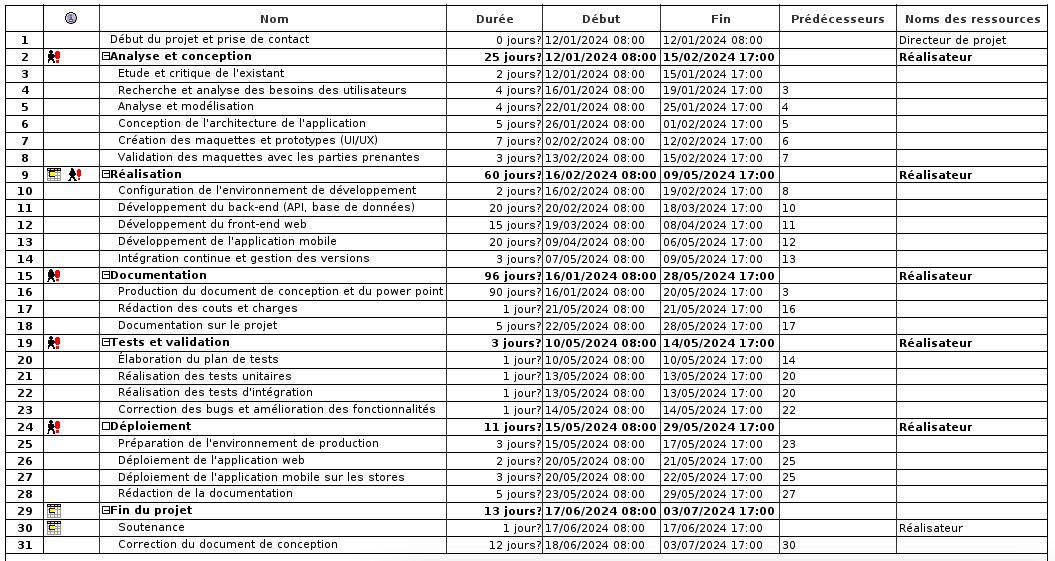
\includegraphics[width=1\textwidth]{capture/task.png}
  \caption{Planification des tâches}
\end{figure}


\section{Diagramme de Gantt}
Le diagramme de Gantt est un outil visuel de gestion de projet qui affiche les
tâches à accomplir sur une ligne de temps. Il permet de suivre les progrès,
d’identifier les dépendances entre les tâches et de prévoir les éventuels retards.

\newpage
% \begin{landscape}
%  \begin{sidewaysfigure}
%   \begin{ganttchart}[
%     hgrid,
%     vgrid,
%     x unit=0.5cm,
%     y unit title=0.7cm, % Augmenter légèrement la hauteur de chaque unité en titre
%     y unit chart=0.7cm, % Augmenter légèrement la hauteur de chaque unité en charte
%     time slot format=isodate,
%     title/.append style={draw=none, fill=gray!30},
%     title label font=\sffamily\bfseries\footnotesize,
%     title height=1,
%     title label anchor/.style={below=-1.6ex},
%     include title in canvas=false,
%     bar label font=\small,
%     bar label node/.append style={align=left},
%     bar/.append style={draw=none, fill=black!63},
%     bar height=0.6,
%     bar top shift=0.2,
%     group top shift=0.4,
%     group height=0.2,
%     group peaks width=0.2,
%     group peaks height=0.2,
%     group peaks tip position=0,
%     group label node/.append style={align=left}
%   ]{2024-05-01}{2024-07-31}
%
%   \gantttitlecalendar{month=shortname} \\
%
%   \ganttgroup{Phase 1}{2024-05-01}{2024-05-31} \\
%   \ganttbar{Task 1}{2024-05-01}{2024-05-15} \\
%   \ganttbar{Task 2}{2024-05-16}{2024-05-31} \\
%
%   \ganttgroup{Phase 2}{2024-06-01}{2024-06-30} \\
%   \ganttbar{Task 3}{2024-06-01}{2024-06-15} \\
%   \ganttbar{Task 4}{2024-06-16}{2024-06-30} \\
%
% \end{ganttchart}
% \end{sidewaysfigure}

% \newgantttimeslotformat{stardate}{%
%   \def\decomposestardate##1.##2\relax{%
%     \def\stardateyear{##1}\def\stardateday{##2}%
%   }%
%   \decomposestardate#1\relax%
%   \pgfcalendardatetojulian{\stardateyear-01-01}{#2}%
%   \advance#2 by-1\relax%
%   \advance#2 by\stardateday\relax%
% }

% \begin{ganttchart}[
%   hgrid,
%   vgrid,
%   time slot format=stardate
%   ]{2259.55}{2259.67}
%   \gantttitlecalendar{year, month=name, week} \\
% \end{ganttchart}

% \begin{ganttchart}[
%     hgrid style/.style={black, dotted},
%     vgrid={*6{black,dotted}, *1{black, dashed}},
%     x unit=3mm,
%     y unit chart=9mm,
%     y unit title=12mm,
%     time slot format=isodate,
%     group label font=\bfseries \Large,
%     link/.style={->, thick}
%     ]{2024-01-01}{2024-06-30}
%
%     % Headers
%     \gantttitlecalendar{year, month=name, week}\\
%
%     % Groupe Analyse des besoins
%     \ganttgroup[
%         group/.append style={fill=orange}
%     ]{Analyse des besoins}{2024-01-01}{2024-02-28} \\ [grid]
%     \ganttorangebar[
%         name=EtudeFonctionnalites
%     ]{Étude des fonctionnalités}{2024-01-01}{2024-01-31} \\ [grid]
%     \ganttorangebar[
%         name=IdentificationExigences
%     ]{Identification des exigences}{2024-01-15}{2024-02-28} \\ [grid]
%
%     % Groupe Conception
%     \ganttgroup[
%         group/.append style={fill=blue}
%     ]{Conception}{2024-02-01}{2024-03-31} \\ [grid]
%     \ganttbluebar[
%         name=ConceptionArchitecture
%     ]{Conception de l’architecture}{2024-02-01}{2024-02-28} \\ [grid]
%     \ganttbluebar[
%         name=ConceptionInterface
%     ]{Conception de l’interface}{2024-03-01}{2024-03-31} \\ [grid]
%
%     % Groupe Développement
%     \ganttgroup[
%         group/.append style={fill=green}
%     ]{Développement}{2024-03-01}{2024-04-30} \\ [grid]
%     \ganttgreenbar[
%         name=ImplementationFonctionnalites
%     ]{Implémentation des fonctionnalités}{2024-03-01}{2024-03-31} \\ [grid]
%     \ganttgreenbar[
%         name=DeveloppementFonctionnalites
%     ]{Développement des fonctionnalités}{2024-04-01}{2024-04-30} \\ [grid]
%
%     % Groupe Tests
%     \ganttgroup[
%         group/.append style={fill=red}
%     ]{Tests}{2024-04-01}{2024-05-31} \\ [grid]
%     \ganttredbar[
%         name=TestsUnitaires
%     ]{Tests unitaires et d’intégration}{2024-04-01}{2024-04-30} \\ [grid]
%     \ganttredbar[
%         name=TestsPerformance
%     ]{Tests de performance}{2024-05-01}{2024-05-31} \\ [grid]
%
%     % Groupe Mise en production
%     \ganttgroup[
%         group/.append style={fill=purple}
%     ]{Mise en production}{2024-05-01}{2024-05-31} \\ [grid]
%     \ganttpurplebar[
%         name=ConfigurationServeurs
%     ]{Configuration des serveurs}{2024-05-01}{2024-05-15} \\ [grid]
%     \ganttpurplebar[
%         name=PublicationApplications
%     ]{Publication des applications}{2024-05-16}{2024-05-31} \\ [grid]
%
%     % Groupe Formation
%     \ganttgroup[
%         group/.append style={fill=brown}
%     ]{Formation}{2024-05-15}{2024-06-30} \\ [grid]
%     \ganttbrownbar[
%         name=FormationUtilisateurs
%     ]{Formation des utilisateurs}{2024-05-15}{2024-05-31} \\ [grid]
%     \ganttbrownbar[
%         name=DocumentationComplete
%     ]{Documentation complète}{2024-06-01}{2024-06-30} \\ [grid]
%
%     % Groupe Maintenance
%     \ganttgroup[
%         group/.append style={fill=gray}
%     ]{Maintenance}{2024-06-01}{2024-06-30} \\ [grid]
%     \ganttgraybar[
%         name=SurveillanceContinue
%     ]{Surveillance continue}{2024-06-01}{2024-06-15} \\ [grid]
%     \ganttgraybar[
%         name=MisesAJour
%     ]{Mises à jour régulières}{2024-06-16}{2024-06-30} \\ [grid]
%
%     % Links
%     \ganttlink[link mid=0.75]{EtudeFonctionnalites}{ConceptionArchitecture}
%     \ganttlink[link mid=0.75]{IdentificationExigences}{ConceptionInterface}
%     \ganttlink[link mid=0.75]{ConceptionArchitecture}{ImplementationFonctionnalites}
%     \ganttlink[link mid=0.75]{ConceptionInterface}{DeveloppementFonctionnalites}
%     \ganttlink[link mid=0.75]{ImplementationFonctionnalites}{TestsUnitaires}
%     \ganttlink[link mid=0.75]{DeveloppementFonctionnalites}{TestsPerformance}
%     \ganttlink[link mid=0.75]{TestsUnitaires}{ConfigurationServeurs}
%     \ganttlink[link mid=0.75]{TestsPerformance}{PublicationApplications}
%     \ganttlink[link mid=0.75]{PublicationApplications}{FormationUtilisateurs}
%     \ganttlink[link mid=0.75]{FormationUtilisateurs}{DocumentationComplete}
%     \ganttlink[link mid=0.75]{DocumentationComplete}{SurveillanceContinue}
%     \ganttlink[link mid=0.75]{SurveillanceContinue}{MisesAJour}
%
% \end{ganttchart}

\begin{figure}[H]
  \centering
  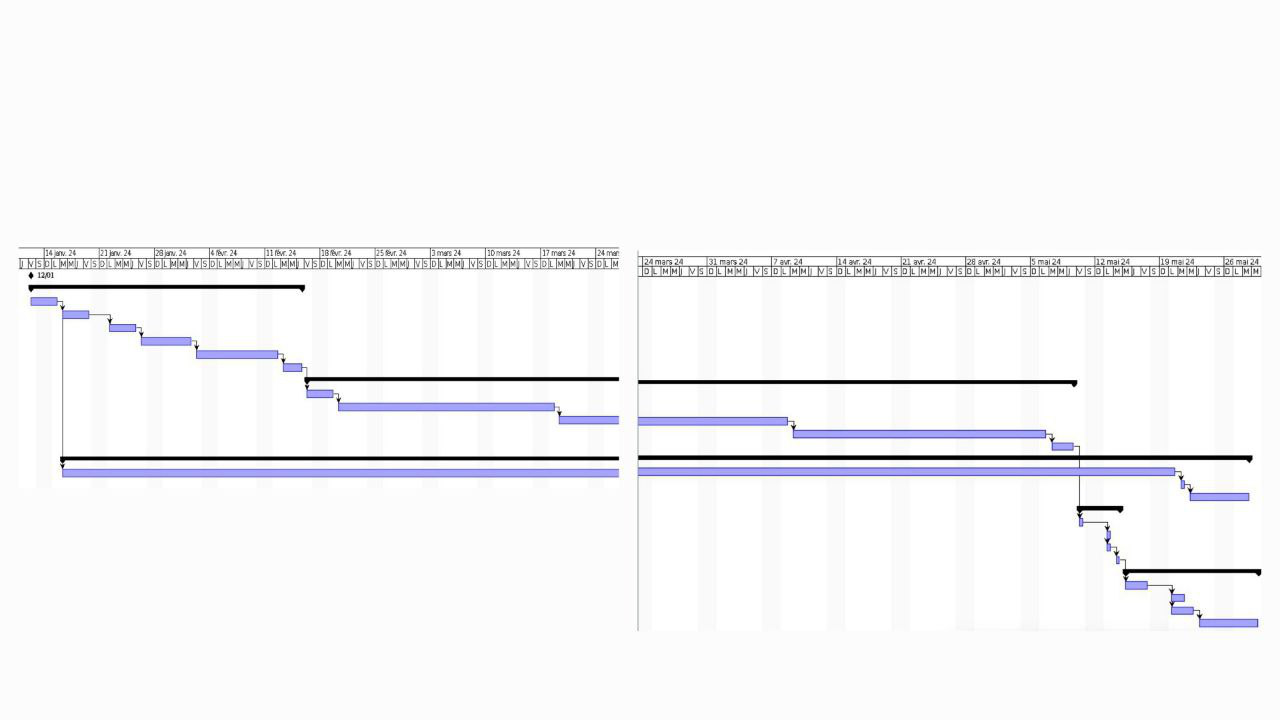
\includegraphics[width=1\textwidth]{capture/gantt.png}
  \caption{Diagramme de Gantt}
\end{figure}



\section{Estimation des charges}
L’estimation des charges implique de calculer le temps et les ressources
nécessaires pour accomplir chacune des tâches du projet.
Des estimations précises sont essentielles pour la planification budgétaire et
la gestion des ressources humaines.


\begin{table}[htbp]
  \centering
  \begin{tabular}{|l|c|c|}
    \hline
    \textbf{Outil et besoin} & \textbf{Quantité} & \textbf{Prix} \\ \hline
    \LaTeX & 1 & 0 FCFA  \\ \hline
    TypeScript & 1 & 0 FCFA  \\ \hline
    Next.js & 1 & 0 FCFA  \\ \hline
    Expo & 1 & 0 FCFA  \\ \hline
    PostgreSQL & 1 & 0 FCFA  \\ \hline
    Docker & 1 & 0 FCFA  \\ \hline
    Git & 1 & 0 FCFA  \\ \hline
    GitHub & 2 & 0 FCFA  \\ \hline
    Neovim & 1 & 0 FCFA  \\ \hline
    VSCodium & 1 & 0 FCFA  \\ \hline
    Figma & 1 & 0 FCFA  \\ \hline
    PC Portable & 2 & 400 000 FCFA  \\ \hline
    Connexion internet & 6 & 25 000 FCFA \\ \hline
    Réalisateurs & 2 & 4 000 000 FCFA \\ \hline
    \multicolumn{2}{|l|}{\textbf{Total}} & \textbf{8 950 000 FCFA} \\ \hline
  \end{tabular}
  \caption{Estimation des charges}
\end{table}

\chapter{Les outils et techniques utilisés}
Ce chapitre présente les outils et les techniques utilisées pour développer
et gérer le projet.

\section{Présentation des techniques}
Les techniques utilisées dans le cadre de ce projet sont les suivantes :

  \textbf{ {Développement Web et Mobile}}

    Pour le développement de la plateforme, nous avons utilisé des techniques
    modernes adaptées au web et aux applications mobiles.
    \begin {itemize}
  \item \textbf{{Next.js}}
    Next.js est un framework React qui permet de créer des applications web côté
    serveur (SSR) et des applications statiques (SSG). Il offre des fonctionnalités
    avancées telles que le rendu côté serveur, le pré-rendu statique, et une
    gestion automatique des routes, ce qui améliore la performance et le
    SEO des applications web.

  \item \textbf{{Expo}}
    Expo est une plateforme et un ensemble d'outils pour le développement
    d'applications mobiles avec React Native. Elle simplifie le processus de
    développement, de déploiement et de mise à jour des applications mobiles,
    tout en offrant des fonctionnalités telles que le rechargement en temps réel,
    l'accès aux API natives et une gestion simplifiée des dépendances.

\end{itemize}

\textbf{{Base de Données}}

  Pour stocker les données de l'application, nous avons utilisé une base de
  données relationnelle PostgreSQL, qui offre des fonctionnalités avancées
  telles que la conformité ACID, la gestion des transactions, et la prise en
  charge de données complexes.

\textbf{{Sécurité}}

  La sécurité est un aspect crucial du développement de la plateforme. Nous
  avons mis en place plusieurs techniques de sécurité pour protéger les données
  des utilisateurs.
  \begin{itemize}
    \item \textbf{{Authentification et Autorisation}}

      Nous avons utilisé un système de session lié à la base de donnée pour
      l'authentification. Les autorisation, pour sécuriser les accès
      à l'application et aux API sont fait par rapport à ces sessions.

    \item \textbf{{Chiffrement des Données}}

      Toutes les communications entre les clients et le serveur sont chiffrées
      en utilisant TLS (Transport Layer Security), garantissant que les données
      transmises restent confidentielles et intactes.
  \end{itemize}

\textbf{Gestion de Projet}

Pour la gestion du projet, nous avons utilisé la méthode objet, qui permet
d'organiser les tâches en fonction de leur importance et de leur priorité.


\section{Présentation des outils}
Les outils utilisés dans le cadre de ce projet sont les suivants :

\textbf{Outils de Développement}
\begin{itemize}
  \item \textbf{Neovim}

    Neovim est un éditeur de texte puissant et extensible, adapté au
    développement de logiciels. Il offre des fonctionnalités avancées telles
    que la coloration syntaxique, la complétion automatique, et la gestion
    des plugins, ce qui améliore la productivité des développeurs.

    \begin{figure}[H]
      \centering
      
\includegraphics[width=0.5\textwidth]{images/Neovim-logo.png}
      \caption{Logo Neovim}
    \end{figure}

  \item \textbf{VSCodium}

    VSCodium est un éditeur de code open-source basé sur Visual Studio Code,
    \begin{figure}[H]
      \centering
      
\includegraphics[width=1.0in, height=1.0in]{images/codium_cnl.png}
      \caption{Logo VSCodium}
    \end{figure}
\end{itemize}

\textbf{Frameworks et Bibliothèques}
\begin{itemize}
  \item \textbf{React}

    React est la bibliothèque JavaScript principale utilisée pour construire
    les interfaces utilisateur de la plateforme web.

  \item \textbf{React Native}

    React Native est le framework JavaScript utilisé pour développer les
    applications mobiles de la plateforme.

    \begin{figure}[H]
      \centering
      
\includegraphics[width=1.0in, height=1.0in]{images/React_Logo_SVG.svg.png}
      \caption{Logo React}
    \end{figure}

  \item \textbf{Next.js}

    Next.js est le framework React utilisé pour le développement côté serveur
    et la génération de sites statiques de la partie web de la plateforme.

    \begin{figure}[H]
      \centering
      
\includegraphics[width=0.5\textwidth]{images/Nextjs-logo.svg.png}
      \caption{Logo Next.js}
    \end{figure}

  \item \textbf{Expo}

    Expo est la plateforme utilisée pour le développement et le déploiement
    des applications mobiles, en fournissant un ensemble d'outils et de
    services pour React Native.

    \begin{figure}[H]
      \centering
      
\includegraphics[width=0.5\textwidth]{images/logo-wordmark.png}
      \caption{Logo Expo}
    \end{figure}

  \item \textbf{shadcn/ui}

    shadcn/ui est une bibliothèque de composants React réutilisables, qui
    permet de créer des interfaces utilisateur cohérentes et esthétiques.
\end{itemize}

\textbf{Outils de Contrôle de Version}
\begin{itemize}
  \item \textbf{Git}

    Git est le système de contrôle de version distribué utilisé pour suivre
    les modifications du code source et faciliter la collaboration entre les
    développeurs.

    \begin{figure}[H]
      \centering
      
\includegraphics[width=0.3\textwidth]{images/Git-logo.svg.png}
      \caption{Logo Git}
    \end{figure}

  \item \textbf{GitHub}

    GitHub est la plateforme utilisée pour héberger le code source et faciliter
    la collaboration via des fonctionnalités comme les pull requests et les
    revues de code.

    \begin{figure}[H]
      \centering
      
\includegraphics[width=1.0in, height=1.0in]{images/GitHub_Invertocat_Logo.svg.png}
      \caption{Logo GitHub}
    \end{figure}
\end{itemize}

\textbf{Outils de Conception}
\begin{itemize}
  \item \textbf{Figma}

    Figma est l'outil de conception utilisé pour créer les maquettes et les
    prototypes de l'interface utilisateur de la plateforme, en facilitant la
    collaboration et le partage des designs.

    \begin{figure}[H]
      \centering
      
\includegraphics[width=1.0in, height=1.2in]{images/800px-Figma-logo.svg.png}
      \caption{Logo Figma}
    \end{figure}

  \item \textbf{\LaTeX}

    \LaTeX est un système de composition de documents utilisé pour rédiger les
    documentations techniques et les rapports. Il offre une mise en
    page professionnelle et une gestion avancée des références. Il permet
    également de créer des diagrammes UML et de toute sorte.

    \begin{figure}[H]
      \centering
      
\includegraphics[width=0.5\textwidth]{images/LaTeX_project_logo_bird.svg.png}
      \caption{Logo \LaTeX}
    \end{figure}
\end{itemize}

\textbf{Outils de Base de Données}
\begin{itemize}
  \item \textbf{PostgreSQL}

    PostgreSQL est le système de gestion de base de données relationnelle
    utilisé pour stocker les données de l'application, en offrant des
    fonctionnalités avancées de gestion des données et de sécurité.

    \begin{figure}[H]
      \centering
      
\includegraphics[width=1.0in, height=1.0in]{images/Postgresql_elephant.svg.png}
      \caption{Logo PostgreSQL}
    \end{figure}

  \item \textbf{Prisma}

    Prisma est un \ac{ORM}  utilisé pour simplifier
    l'accès à la base de données PostgreSQL et faciliter les opérations de
    lecture et d'écriture des données.
    \begin{figure}[H]
      \centering
      
\includegraphics[width=1.0in, height=1.0in]{images/icons8-prisma-orm-500.png}
      \caption{Logo Prisma}
    \end{figure}

  \item \textbf{tRPC}

    tRPC est une bibliothèque de communication entre le client et le serveur
    qui facilite l'appel des API et la gestion des données de manière
    sécurisée et efficace.

    \begin{figure}[H]
      \centering
      
\includegraphics[width=0.5\textwidth]{images/trpc.png}
      \caption{Logo tRPC}
    \end{figure}
\end{itemize}

\textbf{Outils de Sécurité}
\begin{itemize}
  \item \textbf{JWT (JSON Web Tokens)}

    JWT est utilisé pour l'authentification et l'autorisation sécurisées des
    utilisateurs, en générant des jetons d'accès et de rafraîchissement pour
    contrôler l'accès aux ressources de l'application.
    \begin{figure}[H]
      \centering
      
\includegraphics[width=0.5\textwidth]{images/jwt-3026972785.png}
      \caption{Logo tRPC}
    \end{figure}

  \item \textbf{TLS (Transport Layer Security)}

    TLS est utilisé pour chiffrer les communications entre les clients et le
    serveur, en garantissant la confidentialité et l'intégrité des
\end{itemize}

% \item \textbf{Outils de test}
%   \begin{itemize}
%     \item \textbf{Jest}
%
%       Jest est utilisé pour les tests unitaires et les tests d'intégration du
%       code JavaScript et TypeScript.
%
%     \item \textbf{React Testing Library}
%
%       React Testing Library est utilisée pour tester les composants React de
%       manière efficace et fiable.
%   \end{itemize}

\textbf{Outils de conteneurisation}
\begin{itemize}
  \item \textbf{Docker}

    Docker est utilisé pour créer des conteneurs légers et portables qui
    encapsulent les applications et leurs dépendances, facilitant le
    déploiement et la gestion des applications dans différents environnements.

    \begin{figure}[H]
      \centering
      
\includegraphics[width=0.5\textwidth]{images/Docker_logo.svg.png}
      \caption{Logo Docker}
    \end{figure}
\end{itemize}

\textbf{Outils de Déploiement}
\begin{itemize}
  \item \textbf{Vercel}

    Vercel est utilisé pour le déploiement et l'hébergement de la partie web
    de la plateforme développée avec Next.js.

    \begin{figure}[H]
      \centering
      
\includegraphics[width=0.5\textwidth]{images/Vercel_logo_black.svg.png}
      \caption{Logo Vercel}
    \end{figure}

  \item \textbf{Expo Go}

    Expo Go est utilisé pour tester et déployer les applications mobiles
    développées avec Expo et React Native.
\end{itemize}


\section{Les captures d'écrans}
Les captures d’écran illustrent visuellement les étapes importantes du
développement et l’interface utilisateur du produit final. Elles servent à
documenter le travail accompli et à fournir des exemples concrets de
l’application en action.

\begin{figure}[H]
  \centering
  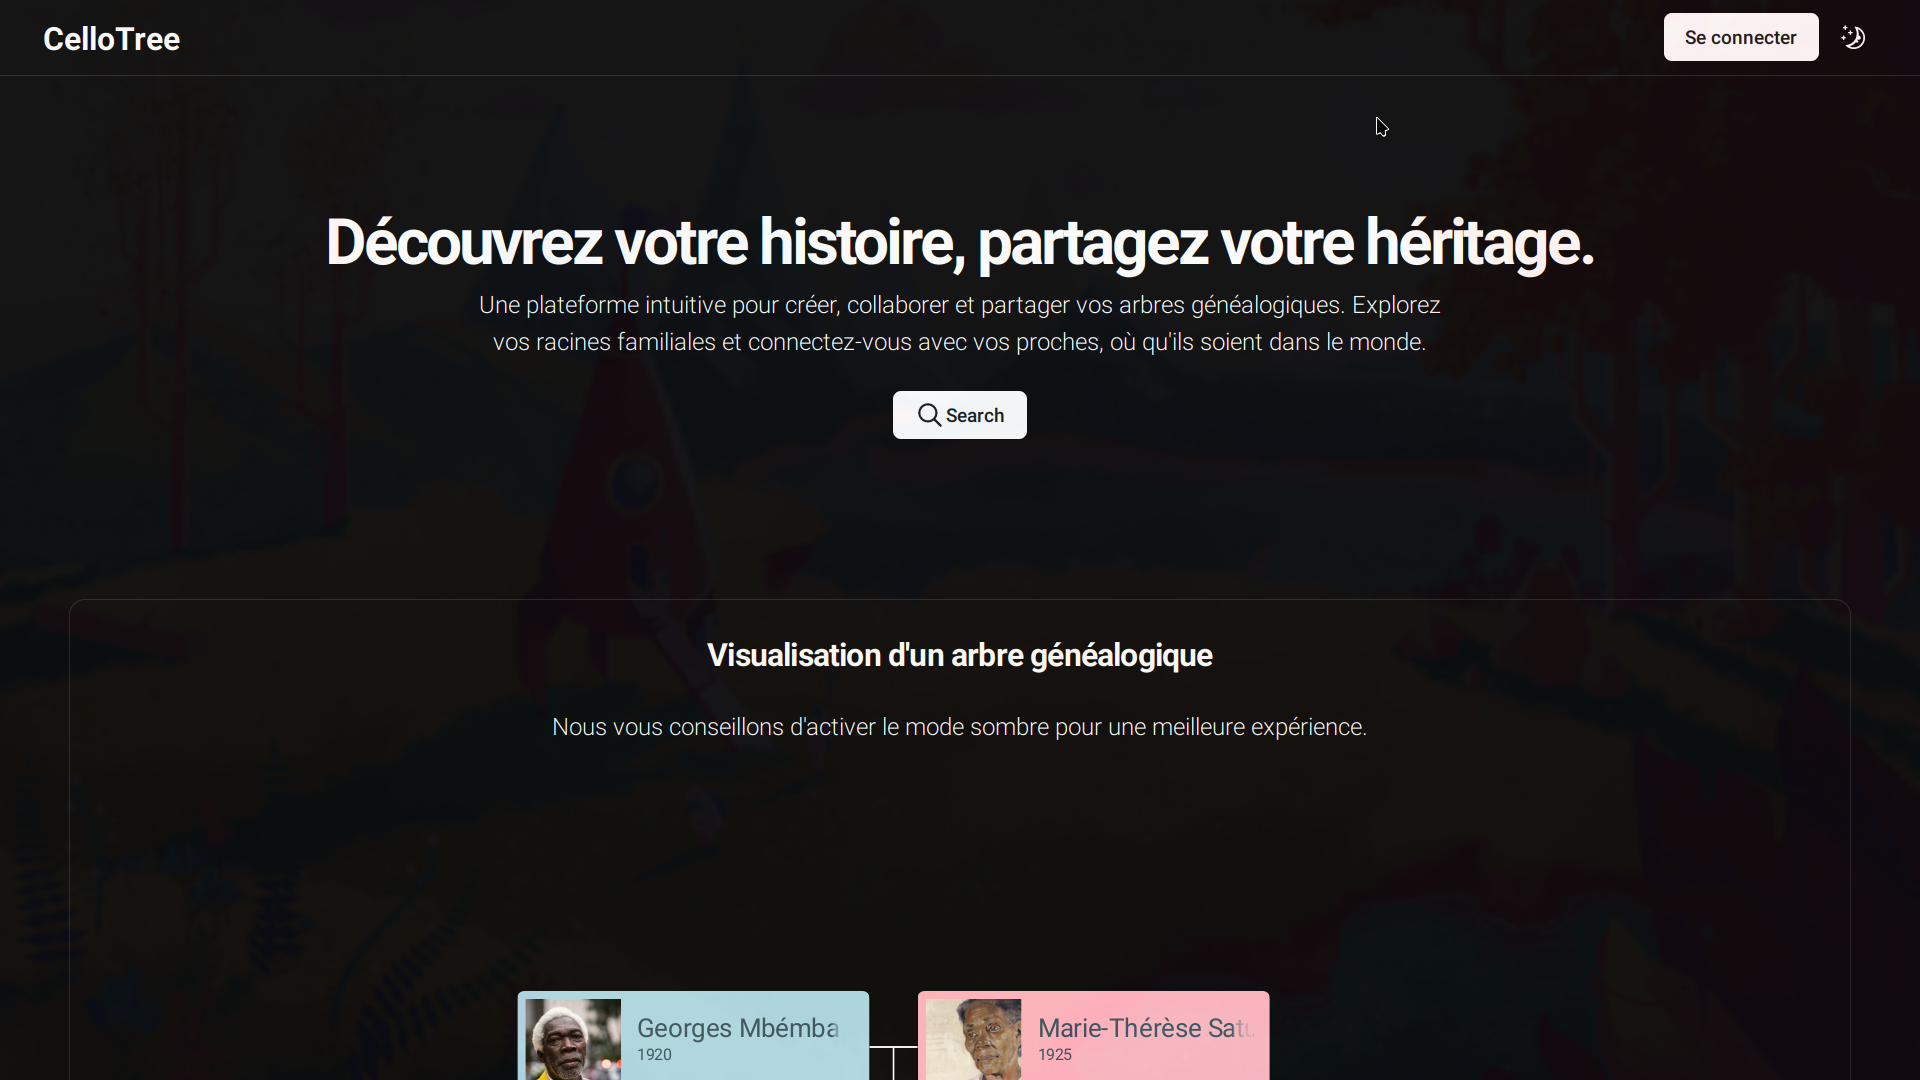
\includegraphics[width=1\textwidth]{./capture/home.png}
  \caption{Écran d'accueil sur l'application web}
\end{figure}

% \begin{figure}[H]
%   \centering
%   \includegraphics[width=0.5\textwidth]{}
%   \caption{Écran d'accueil sur l'application mobile}
% \end{figure}
%
% \begin{figure}[H]
%   \centering
%   \includegraphics[width=0.5\textwidth]{}
%   \caption{Écran de recherche sur l'application web}
% \end{figure}
%
% \begin{figure}[H]
%   \centering
%   \includegraphics[width=0.5\textwidth]{}
%   \caption{Écran de recherche sur l'application mobile}
% \end{figure}
%

\begin{figure}[H]
  \centering
  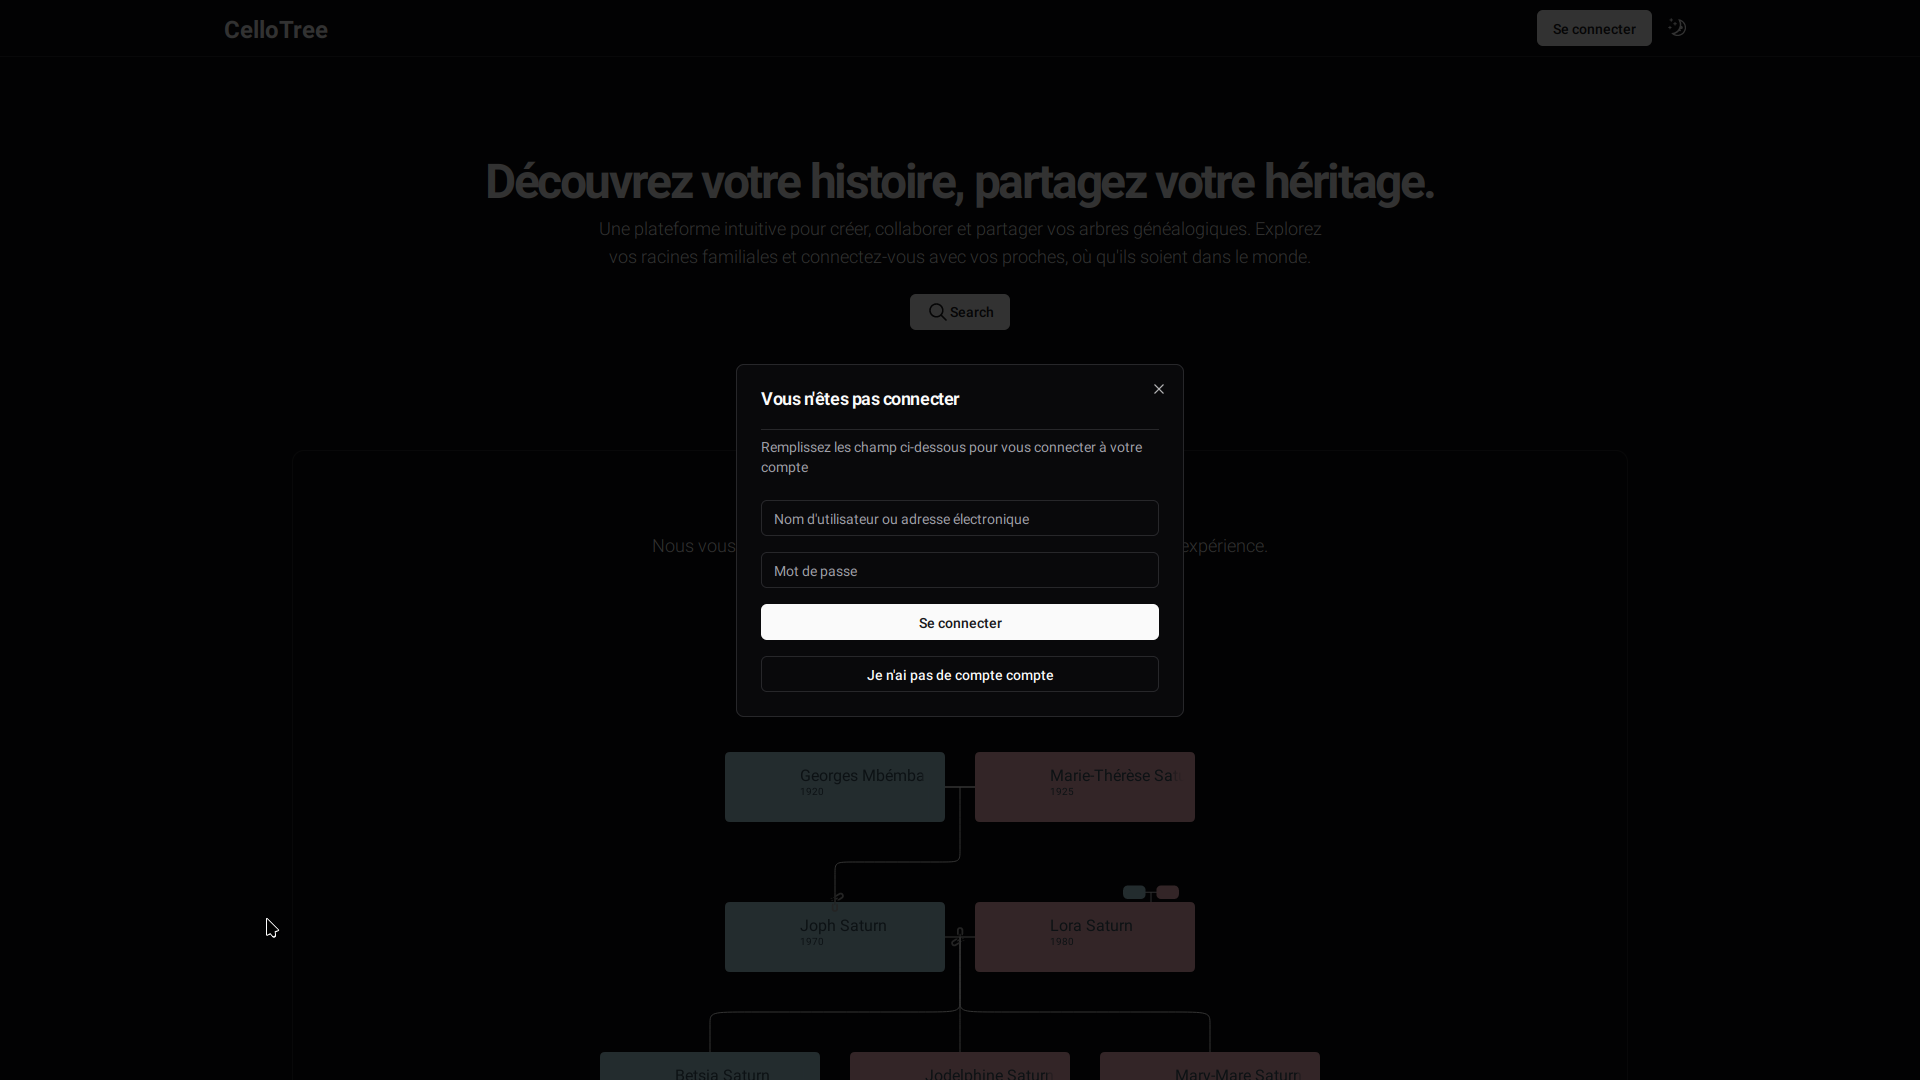
\includegraphics[width=1\textwidth]{capture/login.png}
\caption{Écran de connexion sur l'application web}
\end{figure}

\begin{figure}[H]
  \centering
  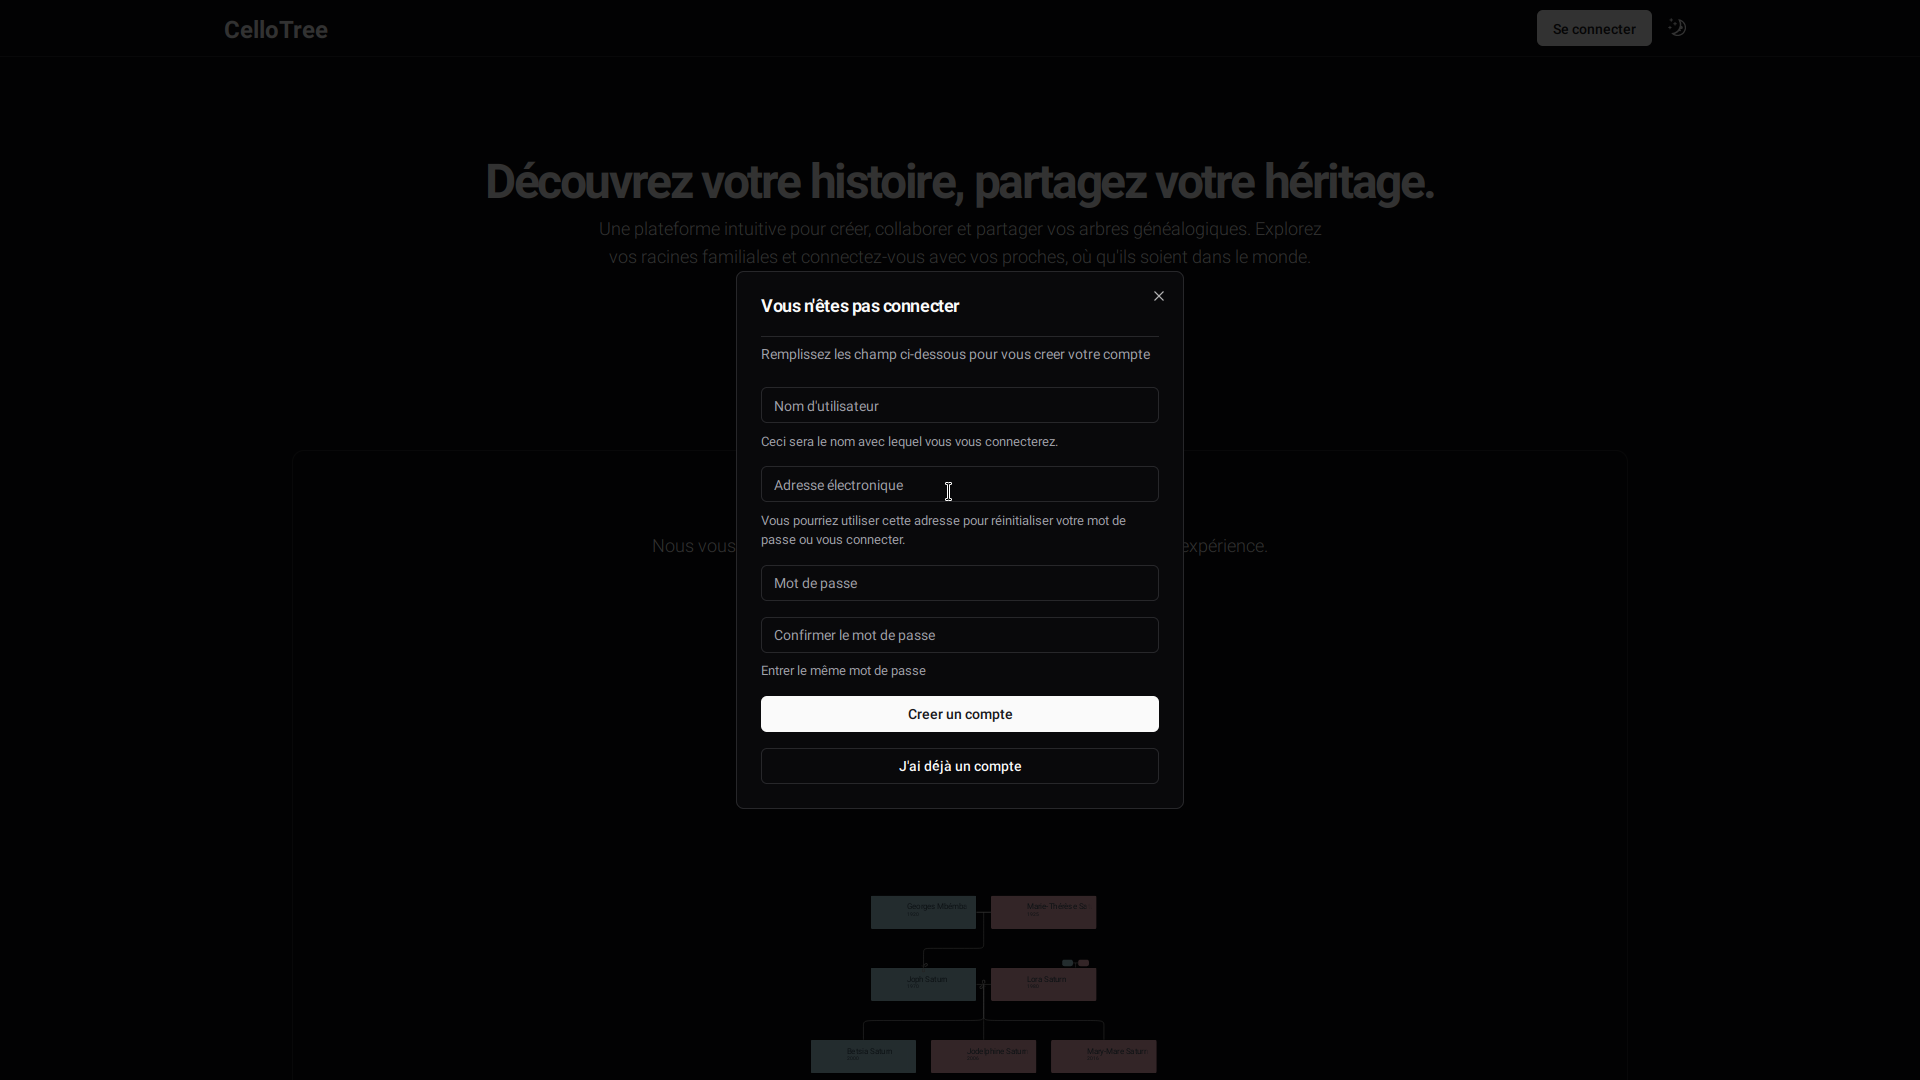
\includegraphics[width=1\textwidth]{capture/signup.png}
  \caption{Écran de création de compte sur l'application web}
\end{figure}

%
% \begin{figure}
%   \centering
%   \includegraphics[width=0.5\textwidth]{}
%   \caption{Écran de connexion sur l'application mobile}
% \end{figure}

\begin{figure}[H]
  \centering
  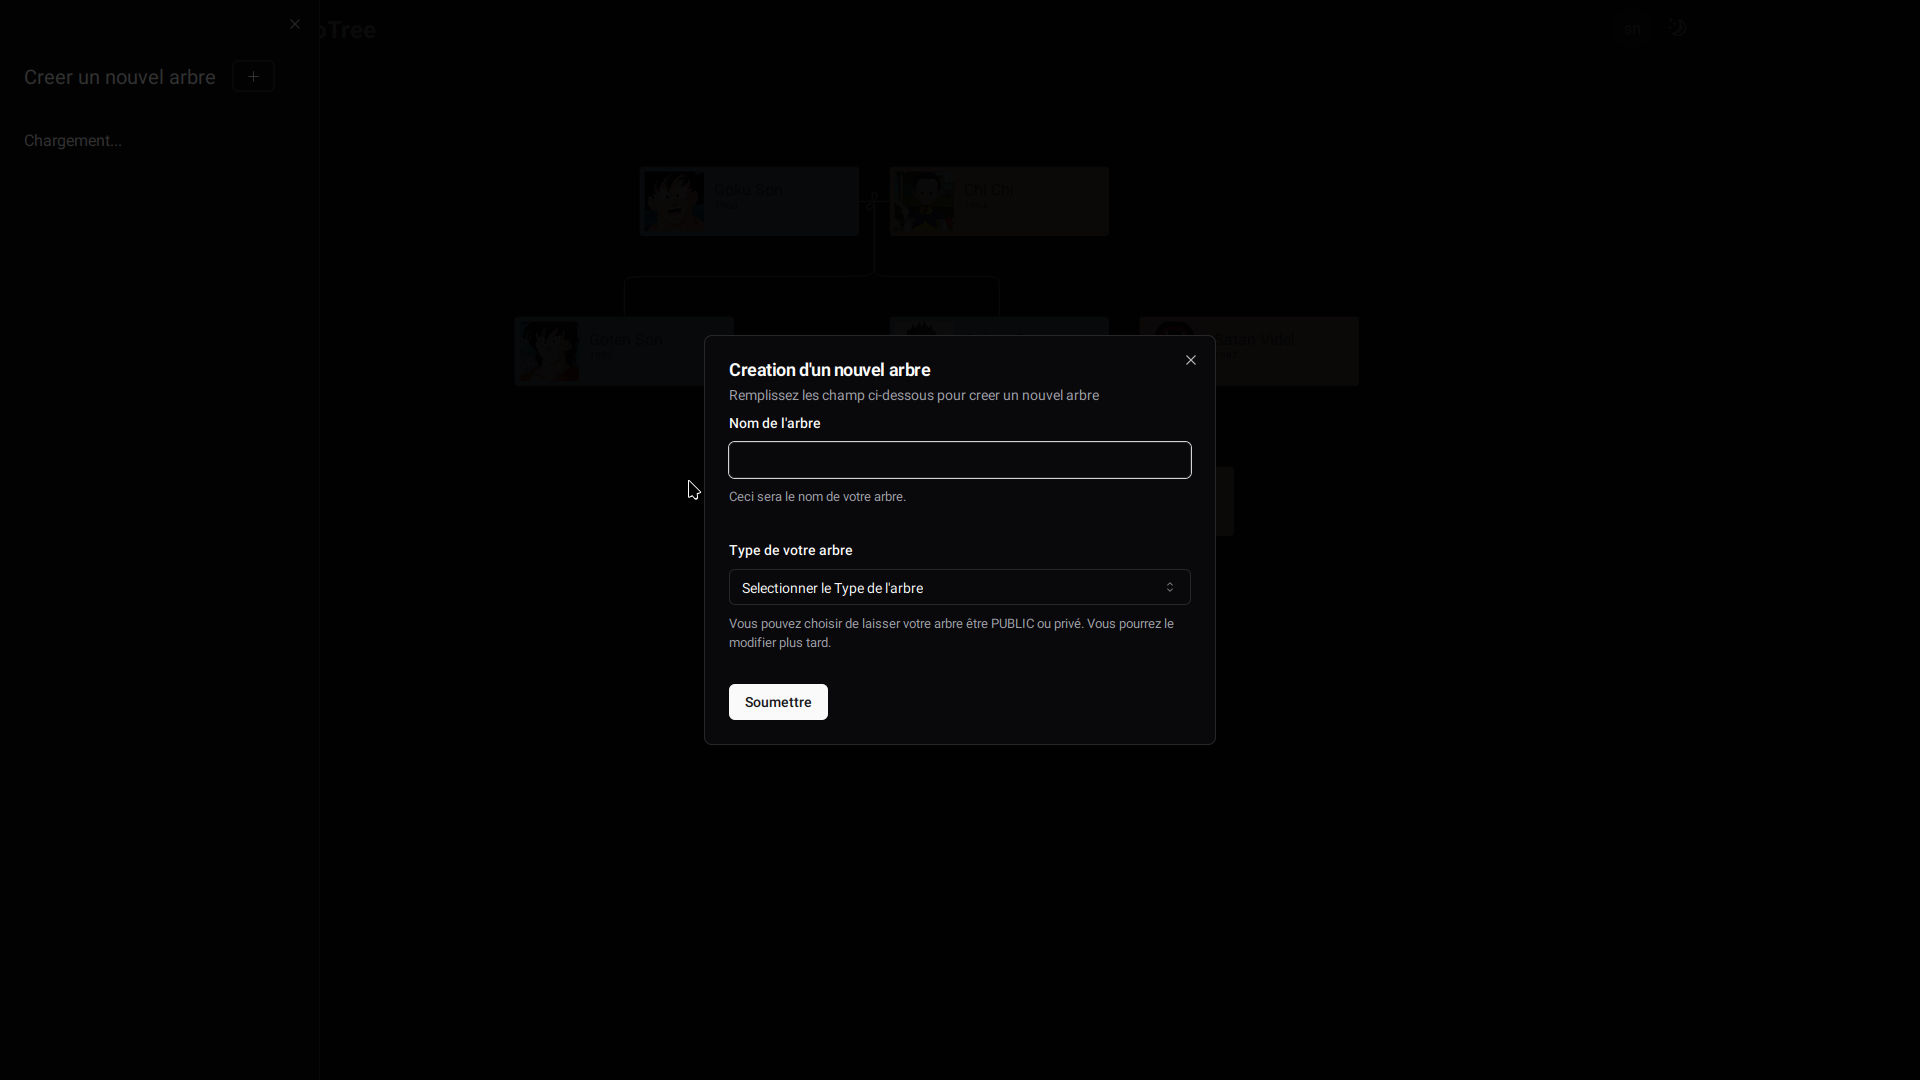
\includegraphics[width=1\textwidth]{capture/tree.png}
  \caption{Écran de création d'un arbre généalogique sur l'application web}
\end{figure}

\begin{figure}[H]
  \centering
  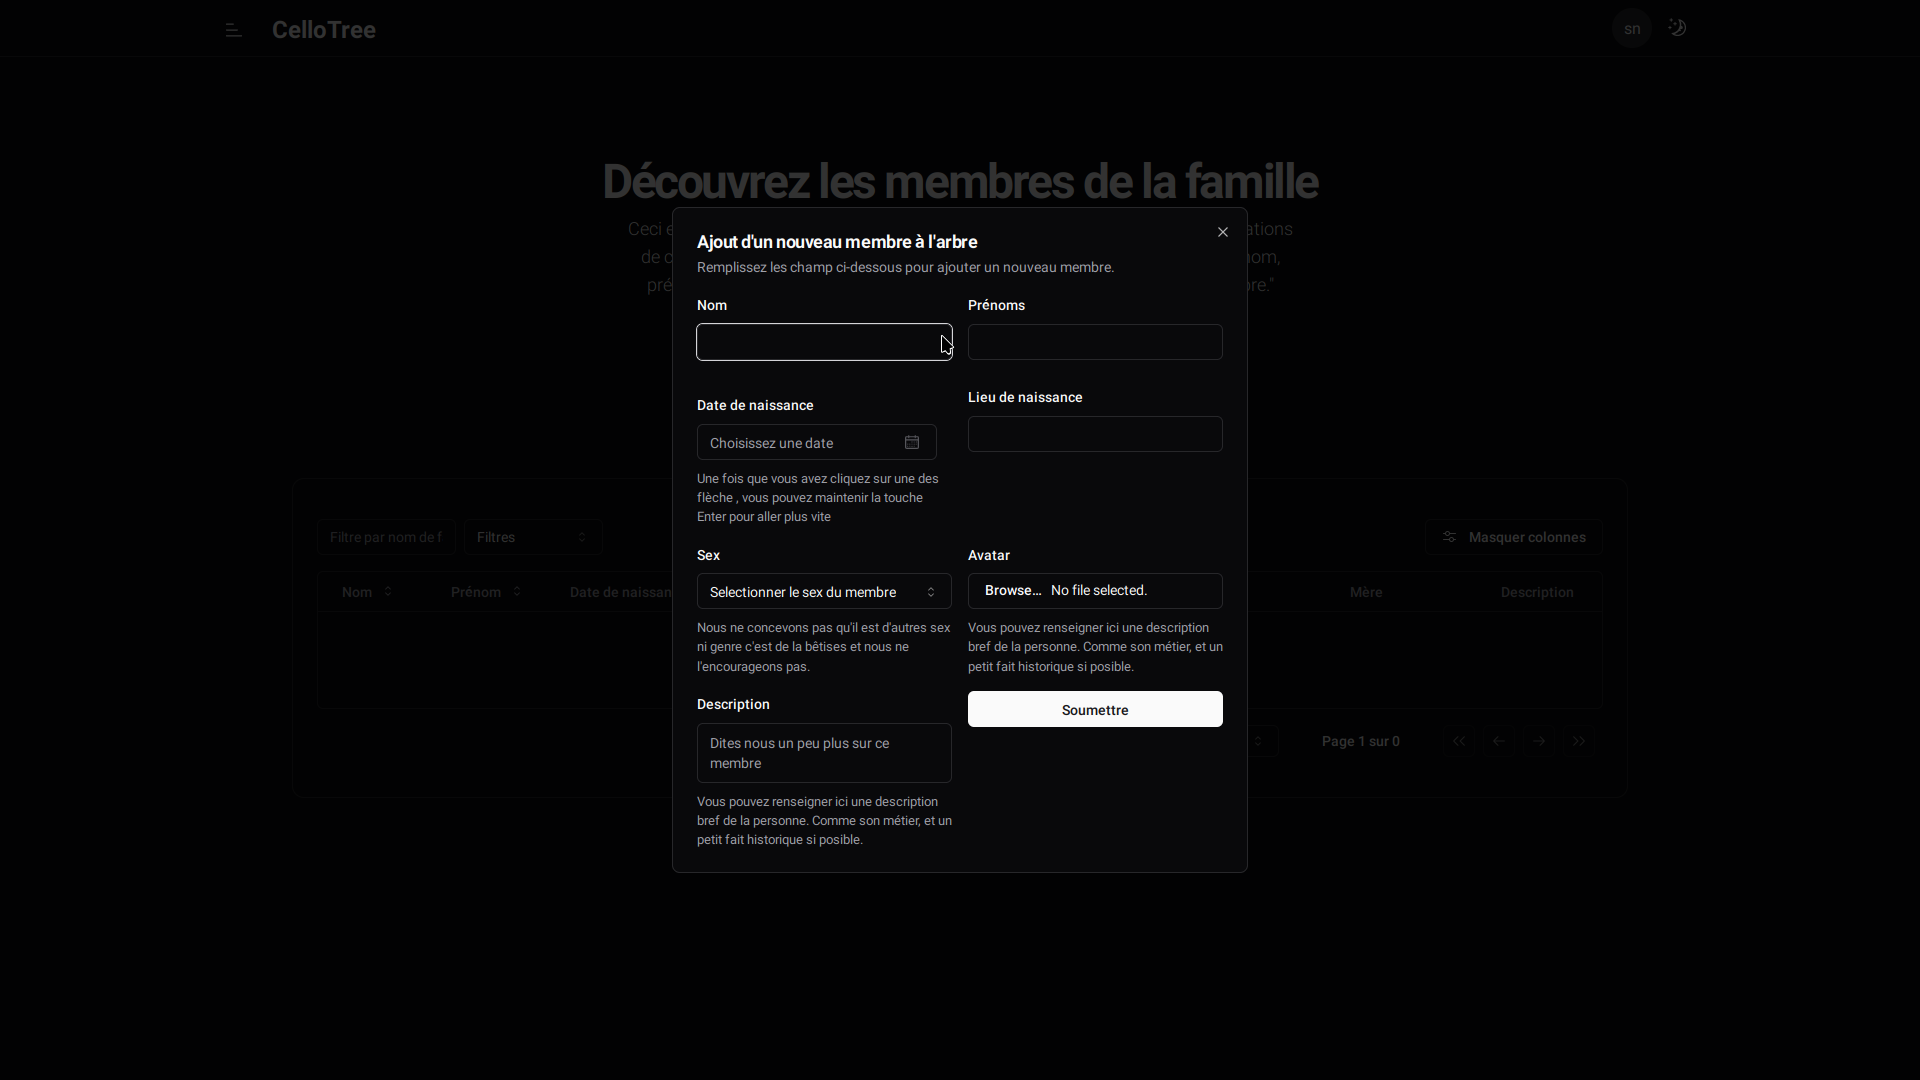
\includegraphics[width=1\textwidth]{capture/member.png}
  \caption{Écran d'ajout d'un membre à un généalogique sur l'application mobile}
\end{figure}

\begin{figure}[H]
  \centering
  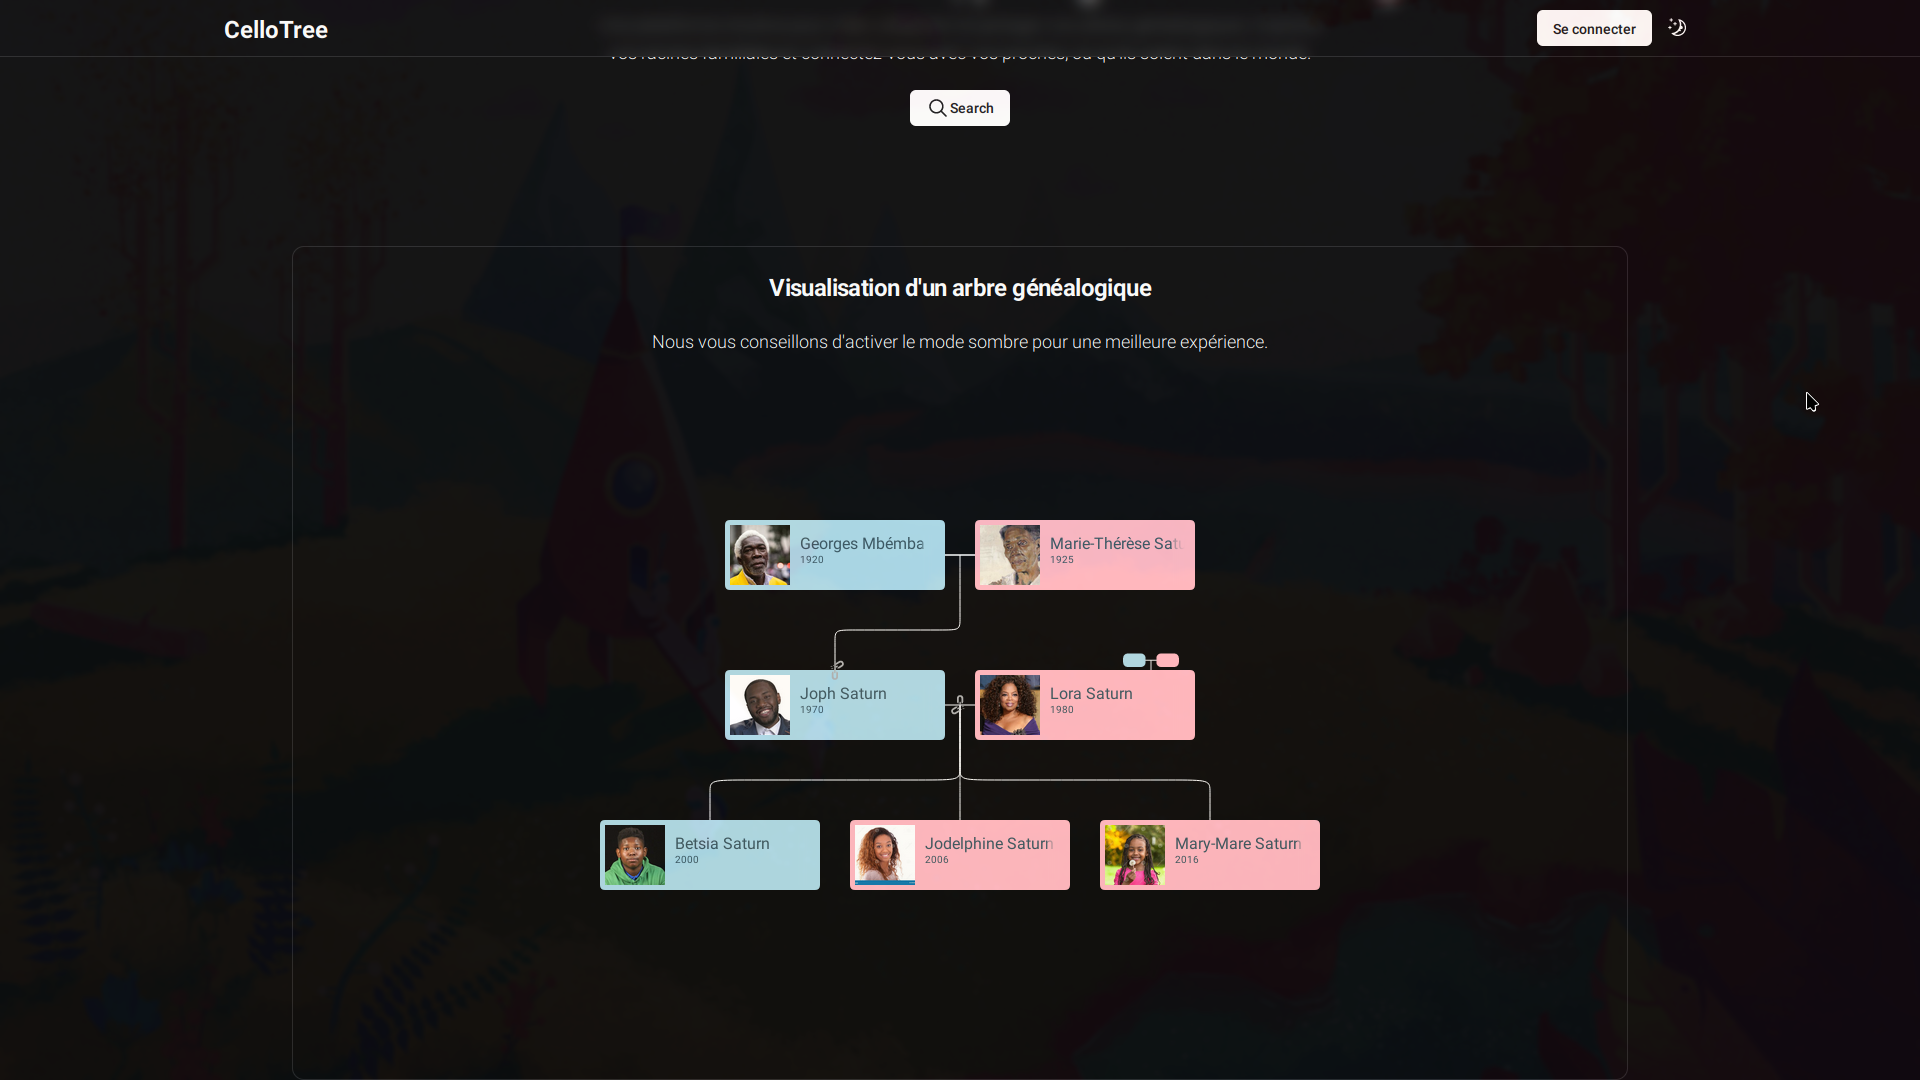
\includegraphics[width=1\textwidth]{capture/view.png}
  \caption{Écran de visualisation d'un arbre généalogique}
\end{figure}

% \begin{figure}[H]
%   \centering
%   \includegraphics[width=0.5\textwidth]{}
%   \caption{Écran de visualisation d'un arbre généalogique sur l'application mobile}
% \end{figure}


\chapter*{Conclusion}
\addcontentsline{toc}{chapter}{Conclusion}
\label{chap:conclusion}
En somme, notre projet de création d’une plateforme web et mobile dédiée à la
généalogie collaborative répond à un besoin croissant de préservation et de
partage de l’héritage familial à l’ère numérique. Il s’inscrit dans une
dynamique de démocratisation de l’accès à la généalogie, permettant à chacun
d’explorer ses racines et de se connecter à son histoire familiale,
indépendamment de ses connaissances préalables ou de sa localisation
géographique.

La méthode objet nous a permis une approche itérative et flexible,
garantissant que la plateforme s’adapte constamment aux besoins des
utilisateurs. Les résultats obtenus jusqu’à présent sont prometteurs et
démontrent l’efficacité de notre approche méthodologique ainsi que la
pertinence des technologies choisies pour le développement de cette solution.

Toutefois, notre travail ne constitue qu’une première étape d’un processus plus
large. Outre les fonctionnalités mises en place, plusieurs questions restent
sans réponse, ouvrant ainsi la porte à de futurs développements. Par exemple :
comment pouvons-nous intégrer des analyses généalogiques avancées pour offrir
des connaissances plus profondes aux utilisateurs? Quelles nouvelles fonctionnalités
pourraient enrichir davantage l’expérience utilisateur, tout en garantissant
la sécurité et la confidentialité des données? Les possibilités sont nombreuses.

En fin de compte, nous espérons que notre plateforme deviendra une référence
incontournable dans le domaine de la généalogie numérique. Elle contribuera
ainsi à la préservation et à la valorisation de l’histoire familiale pour les
générations futures. Ce projet, bien qu’ambitieux, n’est qu’une étape dans la
mission plus large de connecter les individus à leurs racines et de renforcer
le lien familial à travers les outils numériques.


\pagenumbering{Alph}
\label{sec:tableofcontents}
\tableofcontents

\printbibliography
\nocite{roques2004uml}
\label{sec:bibliographie}

\chapter*{Webographie}
\label{sec:webographie}
\addcontentsline{toc}{chapter}{Webographie}
\begin{itemize}
    \item \textbf{Architecture distribuée} \\
    Lien: \url{http://fr.wikipedia.org/w/index.php?title=Architecture_distribu%C3%A9e&oldid=212787328} \\
    Description: Article Wikipédia (encyclopédie libre). \\
    Consulté le : 12-Avril-2024 à 15h00

    \item \textbf{TypeScript Documentation} \\
    Lien: \url{https://www.typescriptlang.org/docs/} \\
    Description: Documentation officielle pour TypeScript, un sur-ensemble typé de JavaScript qui se compile en JavaScript pur. \\
    Consulté le : 16-février-2024 à 09h30

    \item \textbf{Next.js Documentation} \\
    Lien: \url{https://nextjs.org/docs} \\
    Description: Documentation officielle pour Next.js. \\
    Consulté le : 16-février-2024 à 15h45

    \item \textbf{Capacitor} \\
    Lien: \url{https://capacitorjs.com/docs} \\
    Description: Documentation officielle pour Capacitor. \\
    Consulté le : 16-février-2024 à 17h00

    \item \textbf{Prisma Getting Started} \\
    Lien: \url{https://www.prisma.io/docs/getting-started} \\
    Description: Guide de démarrage pour Prisma. \\
    Consulté le : 18-février-2024 à 16h15

    \item \textbf{LaTeX Project Documentation} \\
    Lien: \url{https://www.latex-project.org/help/documentation/} \\
    Description: Documentation officielle du projet LaTeX. \\
    Consulté le : 16-Janvier-2024 à 18h30

    \item \textbf{Lucia Auth Documentation} \\
    Lien: \url{https://lucia-auth.com/} \\
    Description: Documentation pour Lucia. \\
    Consulté le : 03-Mai-2024 à 14h45

    \item \textbf{shadcn/ui Documentation} \\
    Lien: \url{https://ui.shadcn.com/docs} \\
    Description: Documentation pour shadcn/ui. \\
    Consulté le : 16-février-2024 à 19h00

    \item \textbf{Docker Guides} \\
    Lien: \url{https://docs.docker.com/guides/} \\
    Description: Guides et documentation officielle pour Docker. \\
    Consulté le : 27-février-2024 à 19h22

    % \item \textbf{Git Documentation} \\
    % Lien: \url{https://git-scm.com/doc} \\
    % Description: Documentation officielle de Git. \\
    % Consulté le : 16-février-2024 à 12h21

% \item \textbf{TikZ-UML User Guide} \\
    % Lien: \url{https://perso.ensta-paris.fr/~kielbasi/tikzuml/var/files/html/web-tikz-uml-userguide.html} \\
    % Description: Guide utilisateur pour TikZ-UML, une extension de TikZ pour dessiner des diagrammes UML en LaTeX. \\
    % Consulté le : 25-février-2024 à 17h45
\end{itemize}

\end{document}}
